\part{Second-order Refinements: Heavy Tails ($\gamma>0$)}\label{part1}
\chapter{Using Shrinkage Estimators to Reduce Bias and MSE in Estimation of Heavy Tails}\label{chap3}
\setcounter{equation}{0}

\href{https://www.ine.pt/revstat/pdf/Usingshrinkageestimatorstoreducebias.pdf}{\textit{This chapter is based on Beirlant, J., Maribe, G. and Verster, A., 2019. Using shrinkage estimators to reduce bias and MSE in estimation of heavy tails. REVSTAT–Statistical Journal, 17(1), pp.91-108.}}

\section{INTRODUCTION} % --- sections in UPPERCASE
\label{paper1:sec1}       % --- this section label
In this section we consider the estimation of the EVI $\gamma$ and tail probabilities $P(X>x)$ for $x$ large, on the basis of independent and identically distributed observations $X_1, X_2, \ldots, X_n$ which follow a Pareto-type distribution with right tail function (RTF) given by
\begin{equation}
\bar{F}(x) = 1-F(x) = P(X>x) = x^{-1/\gamma} \ell (x)
\label{Patype1}
\end{equation}
where $\ell$ is a slowly varying function at infinity, {\it i.e.}
$$
{\ell (ty) \over \ell (t)} \to 1, \mbox{ as } t \to \infty, \mbox{ for every } y>1.
$$
The most famous estimator of $\gamma$ was first derived by \cite{hill1975simple} as a ML estimator approximating the RTF of the excesses ${X \over t} |X>t$ over a large threshold $t$ by a simple Pareto distribution with RTF $y^{-1/\gamma}$: 
\begin{equation}
\bar{F}(ty)/\bar{F}(t) \approx y^{-1/\gamma}, t \mbox{ large}.
\label{Pot}
\end{equation}
When setting $t= X_{n-k,n}$ where $X_{1,n}\leq X_{2,n} \leq \ldots \leq X_{n,n}$ the ML estimator is given by
\begin{equation}
H_{k,n} = {1 \over k}\sum_{j=1}^k \log {X_{n-j+1,n} \over X_{n-k,n}}.
\label{Hill}
\end{equation}
A simple estimator of a tail probability $P(X>x)$ with $x$ large, introduced in Weissman (1978), is then obtained from \eqref{Pot} setting $ty = x$ and estimating $P(X>t)$ by the empirical proportion $k/n$: 
\begin{equation}
\hat{p}_{x,k} = {k \over n}\left( {x \over X_{n-k,n}}\right)^{-1/H_{k,n}}.
\label{Weiss}
\end{equation}
In practice, a way to verify the validity of model \eqref{Patype1} is to check whether the Hill estimates are stable as a function of $k$. However in most cases the stability is not visible, which can be explained by slow convergence in \eqref{Pot}. For this reason bias reduced estimators have been proposed which lead to plots that are much more horizontal in $k$ which facilitates the analysis of a practical case to a great extent.

\cite{beirlant2009second} proposed a more flexible model capable of capturing the deviation between the true excess RTF $\bar{F}(ty)/\bar{F}(t)$ and the asymptotic Pareto model. For a heavy tailed distribution \eqref{Patype1}, this deviation can be parametrized using a power series expansion \citep{hall}, or more generally via second-order slow variation \citep{bingham1987regular}. 
More specifically in \cite{beirlant2009second} the subclass $\mathcal{F}(\gamma,\tau)$ of the Pareto-type tails \eqref{Patype1} was considered satisfying
\begin{eqnarray}
\bar{F}(x) = C x^{-1/\gamma}\left( 1+\gamma^{-1}\delta (x)\right),
\label{Sclass}
\end{eqnarray}
with $\delta (x)$ eventually nonzero and of constant sign such that $|\delta(x)|=x^\tau \ell_{\delta}(x)$ with $\tau <0$ and $\ell_{\delta}$ slowly varying. 
It was shown that under $\mathcal{F}(\gamma,\tau)$ as $t \to \infty$
$$
\sup_{y \geq 1}\left|{\bar{F}(ty)\over \bar{F}(t)} - \bar{G}_{\gamma,\delta,\tau}(y) \right|
= o\left(|\delta (t)| \right)
$$
with $\bar{G}_{\gamma,\delta,\tau}$ the RTF of the EPD
\begin{equation}
\bar{G}_{\gamma,\delta,\tau}(y)=\{y(1+\delta-\delta y^{\tau})\}^{-1/\gamma}, \ \ \ y>1,
\label{EPD}
\end{equation}
with $\tau <0 < \gamma$ and $\delta > \max (-1,1/\tau)$.
This shows that the EPD improves the approximation \eqref{Pot} with an order of magnitude.
Then ML estimation of the parameters ($\gamma,\delta$) based on a set of excesses 
$\left(Y_{j,k}:=X_{n-j+1,n}/X_{n-k,n},\; j=1,\ldots,k \right)$ was used to obtain a bias reduced estimator $\hat{\gamma}^{ML}_{k,n}$ of $\gamma$. Bias reduction of the Weissman estimator of tail probabilities can analogously be obtained using 
\begin{equation}
\hat{p}^{EP}_{x,k} = {k \over n}\bar{G}_{\hat\gamma _k,\hat\delta _k,\hat\tau}\left( {x \over X_{n-k,n}}\right),
\label{PEP}
\end{equation}
where $(\hat\gamma _k,\hat\delta _k)$ denote the ML estimators based on the EPD model, and where $\hat\tau$ is a consistent estimator of $\tau$, to be specified below, which was shown not to affect the asymptotic distribution of $(\gamma,\delta)$.
\\\\
If $F$ satisfies $\mathcal{F}(\gamma,\tau)$, it is shown in \cite{beirlant2009second} that $U(x):= Q(1-x^{-1})$ ($x>1$), with 
$Q(p) = \inf \{x: F(x) \geq p \}$ ($p \in (0,1)$), satisfies
\begin{equation}
U(x) = C_a{\gamma} x^{\gamma}\left(1+ a(x) \right)
\label{Q}
\end{equation}
with $a(x) = \delta (Q(1-x^{-1}))\{1+o(1)\}= \delta (C_a{\gamma} x^{\gamma})\{1+o(1)\}$ as $x \to \infty$. In particular
$a$ is eventually nonzero and of constant sign and $|a(x)|= x^{\rho}\ell_{a}(x)$ with $\ell_a$ slowly varying and $\rho=\gamma\tau$. Here we assume $|\ell_a (x)|= C_a (1+o(1))$ as $x \to \infty$ for some constant $C_a>0$.
\\\\
The following asymptotic results have been derived for $H_{k,n}$ and $\hat{\gamma}^{ML}_{k,n}$ assuming that $F$ satisfies $\mathcal{F}(\gamma,\tau)$, and $\sqrt{k} a(n/k) \to \lambda \in \mathbb{R}$ and $\hat{\rho}_{k,n} = \rho + o_p(1)$ as $k,n \to \infty$ and $k/n \to 0$, the following asymptotic results hold for the EPD-ML estimator $\hat{\gamma}^{ML}_{k,n}$ and $H_{k,n}$:
\begin{eqnarray}
\sqrt{k} \left( H_{k,n}-\gamma \right) & \to^d & 
\mathcal{N}\left(\lambda {\rho \over 1-\rho} , \gamma^2
\right), \label{limH} \\ 
\sqrt{k} \left( \hat{\gamma}^{ML}_{k,n}-\gamma \right) & \to^d & 
\mathcal{N}\left(0, \gamma^2 \left({1-\rho \over \rho} \right)^2
\right).
\label{limML} 
\end{eqnarray}
An estimator $\hat{\rho}_{k,n}$ of $\rho$ can be taken from \cite{alves2003new} using $k=k_1= \lfloor n^{1-\epsilon}\rfloor$ for some $\epsilon >0$ (see, Appendix \ref{appendix1b}). The required consistency for $\hat{\rho}_{k,n}$ was obtained under \eqref{Q}.
\\\\
Asymptotic results of the type \eqref{limH} and \eqref{limML} are typical for bias reduced estimators when both $\gamma$ and $a(n/k)$ or $\delta$ are jointly estimated at every $k$ value:
for larger values of $k$ corresponding to $\sqrt{k} a(n/k) \to \lambda \neq 0$, bias reduced estimators still have asymptotic bias 0 in contrast to the Hill estimator, but their variance is increased by a factor $((1-\rho)/\rho)^2$ compared to $H_{k,n}$.
\\\\
In a pioneering paper, \cite{caeiro2005direct} proposed to estimate $(n/k)^{-\rho} a(n/k)$ at a high level $k=k_1= \lfloor n^{1-\epsilon}\rfloor$, leading to a corrected Hill estimator (denoted below by $CH_{k,n}$) with asymptotic variance $\gamma^2$ and excellent bias and MSE characteristics. To obtain the normal asymptotic behaviour of such minimum variance reduced bias estimators one needs a third-order slow variation condition which is more restrictive than \eqref{Q} or condition $\mathcal{F}(\gamma,\tau)$.  

\vspace{0.3cm}\noindent
Up to now, to the best of our knowledge, the fact that $\delta (t) \to 0$ as $t \to \infty$, or $a(n/k)\to 0$ as $n/k \to \infty$ has not been exploited in the literature. However, this calls for shrinkage estimators.
Such shrinkage approach can be implemented by putting a penalty on $\delta$ in an ML procedure, leading to penalised ML. Alternatively a penalty on $\delta$ can be naturally introduced in a Bayesian approach putting an appropriate prior on this parameter. 
\\\\
Here we investigate the use of shrinkage estimation when modelling the distribution of the vector of excesses ${\bf Y}_k := \left( Y_{j,k}, j=1,\ldots,k \right)$
with an EPD. In \autoref{chap3::sec2} we show that a quadratic penalty, or equivalently a normal prior, on $\delta$ with zero mean and variance $\sigma^2_{k,n}$, depending in an appropriate way on $k$ and $n$, leads to interesting asymptotic MSE results for $\gamma$. In \autoref{chap3::simulation} we 
consider the finite sample behaviour of the penalised likelihood and Bayes approach, and make a comparison with the minimum variance reduced bias estimator, and consider a practical case. 

\section{Shrinkage estimators of the EPD parameters}\label{chap3::sec2}

\subsection{penalised likelihood and Bayesian interpretation}
ML estimation of the EPD parameters ($\gamma,\delta$), given a value of $\tau$, follows by maximising the log-likelihood
\begin{eqnarray}
{1 \over k}l_{EP}(\gamma,\delta |{\bf y}) &=& -\log \gamma
-(\frac{1}{\gamma}+1){1 \over k}\sum_{j=1}^k\left[\log y_{j,k} + \log(1+\delta\{1-y_{j,k}^{\tau}\})\right] \nonumber \\&&
+{1 \over k}\sum_{j=1}^k\log\left(1+\delta\{1-(1+\tau)y_{j,k}^{\tau}\}\right).
\label{logl}
\end{eqnarray}
Shrinkage estimators are then obtained by putting a penalty on $\delta$. Below it will be shown that a quadratic penalty is appropriate in view of the asymptotic results for the penalised maximum likelihood (PML) estimators $(\hat{\gamma}_{k,n}^{P},\hat{\delta}^P_{k,n})$. These estimators are then obtained by optimising the log-likelihood
\begin{equation}
{1 \over k}l_{pen} (\gamma,\delta |{\bf y}) = {1 \over k}l_{EP}(\gamma,\delta |{\bf y}) - \omega {\delta^2 \over 2k\sigma_{k,n}^2}, 
\label{loglp}
\end{equation}
where $\omega >0$ serves as a tuning constant regulating the amount of penalty, and $\sigma_{k,n}^2$ indicating the penalty rate as a function of $k$. From the asymptotic analysis below, it follows that $\sigma^2_{k,n} = (k/n)^{-2\rho}$ is appropriate. 
\\\\
Alternatively, from a Bayesian perspective, a shrinkage estimator is obtained by considering the posterior mode estimators $(\hat{\gamma}_k^{B},\hat{\delta}_k^B)$ of the log-posterior
\begin{equation}
{1 \over k} \log p (\gamma,\delta|{\bf y}) = 
{1 \over k}l_{EP}(\gamma,\delta |{\bf y}) + {1 \over k}\log \pi (\gamma,\delta),
\label{logpost}
\end{equation}
where $\pi (\gamma,\delta)$ denotes the prior density on $(\gamma,\delta)$. In correspondence with the choice for the penalised log-likelihood \eqref{loglp}, we here choose a normal prior on $\delta$ with mean 0 and variance $\sigma^2_{k,n}$. We also truncate it from the left in order to comply with the restriction
$\delta > \max (-1,1/\tau)$:
\begin{equation}
\pi (\delta) = {1 \over \sqrt{2\pi}\sigma_{k,n}}e^{-{1 \over 2}{\delta^2 \over \sigma^2_{k,n}}}/ \left( 1-\Phi (\max (-1,\tau^{-1})/\sigma_{k,n})\right).
\label{pidelta}
\end{equation} 

\subsection{Asymptotic results for the penalised ML estimator $\hat{\gamma}^P_k$}

In Appendix \ref{appendix1} we derive that the first order approximations ($\gammab,\db$) of the penalised ML estimators are given by
\begin{eqnarray*}
	\gammab & =& H_{k,n} +\db \left( 1-E_{k,n}(\tau) \right) ,\\
	\db &=& \frac{1-H_{k,n}\tau}{D^{P}_{k,n}} \left(E_{k,n}(\tau) - {1 \over H_{k,n}\tau} \right)
\end{eqnarray*}
where 
$$
E_{k,n}(s) = {1 \over k}\sum_{j=1}^k Y_{j,k}^{s},\; s < 0,
$$
and 
\begin{eqnarray*}
D^{P}_{k,n} =
{\omega \gammab \over k\sigma^2_{k,n}} -
 \Big(1 &-& 2(1-\gammab \tau) E_{k,n}(\tau)+ (1-2\gammab\tau-\gammab\tau^2)E_{k,n}(2\tau) \\ 
&-& \tau (1- E_{k,n}(\tau))E_{k,n}(\tau)\Big).
\end{eqnarray*}
These expressions are identical to the asymptotic EPD-ML estimators derived in \cite{beirlant2009second} except for the extra term ${\omega \gammab\over k\sigma^2_{k,n}}$ in the expression of $D^{P}_{k,n}$. 
As an external estimator of $\tau$ we use $\hat{\tau} = \hat{\rho}_{k,n}/H_{k,n}$ with $\hat{\rho}_{k,n}$ taken from \cite{alves2003new}. Moreover we set $\zeta=\gamma^2 (1-2\rho)(1-\rho)^2$. The following result is derived in Appendix \ref{appendix1}. 
\\
\begin{theorem}\label{theorem11} {\it Let $F \in \mathcal{F}(\gamma,\tau)$ with $|a(x)| =x^{\rho }C_a (1+o(1))$ as $x \to \infty$. Assume that $\sqrt{k} a(n/k) \to \lambda$ as $k,n \to \infty$, $k/n \to 0$. Setting $\sigma_{k,n}^2= (k/n)^{-2\rho}$, it follows that $\gamma_{k,n}:=\sqrt{k} \left( \gammab-\gamma \right)$ is asymptotically normal with asymptotic mean and variance given by
	\begin{eqnarray}
	E_{\infty} (\gamma_{k,n}) &=& 
	{\lambda \rho \over 1-\rho}{\zeta C_a^2 \omega \over \zeta C_a^2 \omega + \rho^4 \lambda^2}, 
	\label{Abias}\\
	Var_{\infty} (\gamma_{k,n})&=& {\gamma^2 \rho^8\lambda^4 \over (\rho^4\lambda^2+ \zeta C_a^2 \omega )^2}\left( \left({1-\rho \over \rho} \right)^2
	+ {\zeta^2 C_a^4 \omega^2 \over \rho^8 \lambda^4}+ 2{\zeta C_a^2 \omega \over \rho^4 \lambda^2}\right). 
	\label{Avar}
	\end{eqnarray}
	$\blacktriangle$
}
\end{theorem}

\vspace{0.3cm}\noindent
Minimising $MSE_{\infty}(\gamma_{k,n})= E^2_{\infty} (\gamma_{k,n})
+ Var_{\infty} (\gamma_{k,n})$ 
with respect to $\omega$, this leads to the asymptotically optimal value (see Appendix \ref{appendix1a}) $$\omega_{opt}= C_a^{-2}.$$ 
One then obtains from \eqref{Abias} and \eqref{Avar} that 
\begin{eqnarray*}
	E^{opt}_{\infty} (\gamma_{k,n}) &=& {\lambda \rho\over 1-\rho}
	{\zeta \over \zeta + \lambda^2 \rho^4 },\\
	Var^{opt}_{\infty} (\gamma_{k,n}) &=& {\gamma^2 \over (\lambda^2\rho^4+ \zeta)^2}
	\left\{(1-\rho)^2\rho^6 \lambda^4 + \zeta^2 + 2\zeta \rho^4\lambda^2 \right\},
\end{eqnarray*}
from which 
\begin{equation}
MSE^{opt}_{\infty}(\gamma_{k,n}) =
\gamma^2 + { \lambda^2 \rho^2 \gamma^2 (1-2\rho) \over \gamma^2 (1-2\rho)(1-\rho)^2 + \rho^4 \lambda^2}.
\label{xisqdiff}
\end{equation}
Since the right hand side of \eqref{xisqdiff} is an increasing function in $\lambda^2$ it follows that
$$
MSE^{opt}_{\infty}(\gamma_{k,n}) \leq \lim_{\lambda \to \infty}MSE^{opt}_{\infty}(\gamma_{k,n}) = MSE_{\infty}\left(\sqrt{k}(\hat{\gamma}_{k,n}^{ML}-\gamma)\right)= \gamma^2 ({1-\rho \over \rho})^2.
$$ 
Also, expanding the right hand side of \eqref{xisqdiff} for $\lambda^2 \to 0$ leads to 
$$
MSE^{opt}_{\infty}(\gamma_{k,n}) = \gamma^2 + \lambda^2 {\rho^2 \over (1-\rho)^2}(1+o(1)).
$$
We can conclude that the asymptotic MSE of the optimal penalised estimator is uniformly smaller than the MSE of the EPD-ML estimator as given in \eqref{limML}, while for smaller $\lambda$ this asymptotic MSE follows the asymptotic MSE of the Hill estimator, given in \eqref{limH}, up to terms of order $\lambda^2$. Hence with the penalty $\omega /\sigma^2_{k,n}= C_a^{-2}(k/n)^{2 \rho}= a^{-2}(n/k)$ in \eqref{loglp}, the penalised ML estimator asymptotically follows the better of the two existing estimators as a function of $\lambda$ or $k$.
\\\\
Replacing ($\hat\gamma _k,\hat\delta _k$) by ($\hat\gamma ^{P}_k,\hat\delta ^{P}_k$) in $\hat{p}^{EP}_{x,k}$, it follows from the proof of Theorem 5.2 in \cite{beirlant2009second} that the resulting tail probability estimator $\hat{p}^{P}_{x,k}$ satisfies the following asymptotic result under the conditions of the Theorem: \\
when $p_n = P(X>x_n)$ satisfies $np_n/k \to 0$ and $\log(np_n)/\sqrt{k} \to 0$, then 
$${\sqrt{k} \over \log (k/(np_n))}\gamma ( {\hat{p}^{P}_{x_n,k} \over p_n}-1)$$ is asymptotically normal with the same limit distribution as in the Theorem. Hence the asymptotic MSE behaviour for the tail probability estimator has the same characteristics as the tail index estimator.
\\\\
From the simulations it will follow that the choice $\omega =1$ and the use of estimator of $\rho$ taken from \cite{alves2003new} yields good results. However, in order to alleviate the problem of choosing the number of top order statistics $k$ that are used in the estimation procedure, one can choose $\omega$ adaptively with each sample aiming for a plot of $\hat{\gamma}^P_k$ as a function of $k$ which is as horizontal as possible. Setting $\hat{\gamma}_k^P =\hat{\gamma}_k^P (\omega)$ in order to emphasise the dependence of the penalised ML estimator on $\omega$, a possible choice of $\omega$ is obtained by minimising the variance of the resulting estimators for $k=1,\ldots,n$:
\begin{equation}
\omega_{mv} = \mbox{argmin}_{\omega} s^2_n \left(\hat{\gamma}^P (\omega)\right),
\label{minvar}
\end{equation}
with $s^2_n (\hat{\gamma}^P (\omega)) = {1 \over n-1}\sum_{k=1}^n \left( \hat{\gamma}_k^P (\omega) - \bar{\hat{\gamma}}^P\right)^2$.


\section{Simulations and practical case studies}\label{chap3::simulation}

Both the Bayes maximum a posteriori probability estimator and the penalised maximum likelihood estimator are implemented in \textbf{R} using the general \textbf{optim} function with default parameters. 

\noindent We performed a simulation study, taking 1000 repetitions of samples of size $n=200, 500, 1000$ studying the finite sample behaviour of $\hat{\gamma}^P_{k,n}(\omega)$  for different distributions. The bias and root mean squared error (RMSE) are plotted as a function of $k$. 
\\\\
The following distributions are used:
\begin{itemize}
	\item 
	{\it The extreme value distribution} (EV) with
	$F(x)= \exp (-(1+\gamma x)^{-1/\gamma})$ $(1+\gamma x >0)$ taking $\gamma=0.25$ in which case $\rho=-0.25$ and $C_a=1$.
	\item
	{\it The Fr\'echet distribution} with $\bar{F}(x)= 1-\exp(-x^{-1/\gamma})$ taking $\gamma = 0.5$ in which case $\rho=-1$ and $C_a=0.25$.
	\item
	{\it The Burr distribution} with $\bar{F}(x)= (1+x)^{-4/3}$ so that $\gamma = 0.75$ and $\rho=-0.75$ and $C_a=1$.
	\item
	{\it The loggamma distribution} with $\bar{F}(x) \sim constant \times x^{-2}(\log x)^3$ so that $\gamma = 0.5$, which does not belong to the class $\mathcal{F}(\gamma,\tau)$.
\end{itemize}
First in Figures \ref{paper1:fig1}-\ref{paper1:fig4} we plotted the bias and the RMSE of the Hill estimator $H_{k}$, the EPD-ML estimator $\hat{\gamma}_{k}^{ML}$, the penalised ML estimator $\hat{\gamma}^P_{k}(1)$ with $\omega=1$, the Bayesian estimator $\hat{\gamma}^B_{k}(1)$ with $\omega=1$, and the minimum variance reduced bias estimator $CH_k$ from Caeiro {\it et al.} (2005) given by
\[
CH_k = H_{k,n}\left( 1- {\hat{\beta}_{k_1} (\hat{\rho}_{k_1}) \over 1- \hat{\rho}_{k_1}}\left({n \over k} \right)^{\hat{\rho}_{k_1}}\right),
\] 
with 
\[
\hat{\beta}_k (\rho) =
\frac{ \left({k \over n} \right)^{\rho} 
\left\{ \left({1 \over k} \sum_{j=1}^k ({j \over k})^{-\rho}\right) \left({1 \over k} \sum_{j=1}^k Z_j\right) 
-\left({1 \over k} \sum_{j=1}^k ({j \over k})^{-\rho} Z_j\right) 
\right\} }
{\left({1 \over k} \sum_{j=1}^k ({j \over k})^{-\rho} \right) \left({1 \over k} \sum_{j=1}^k ({j \over k})^{-\rho} Z_j\right) -\left({1 \over k} \sum_{j=1}^k ({j \over k})^{-2\rho} Z_j\right) },
\]
where $Z_j := j(\log X_{n-j+1,n}-\log X_{n-j,n})$ $(j=1,2,\ldots)$, and $k_1 = \lfloor n^{0.99}\rfloor$. 

\noindent In Figure \ref{paper1:fig5} we briefly report on the effect of the choice of $\omega$ using $\omega=1$ and $\omega= \omega_{mv}$ and compare these with the optimal asymptotic RMSE expression from \eqref{xisqdiff}.

\noindent We conclude from the simulations that the finite sample behaviour of the proposed estimators follows the characteristics predicted by the asymptotic analysis to a great extent: for small $k$ the shrinkage estimators
$\gamma_{k}^P$ and $\gamma_{k}^B$ show a similar behaviour as the Hill estimator, while for larger $k$ the proposed estimators tend to follow the characteristics of the bias reduced EPD-ML estimator. In between these two $k$-regions the shrinkage estimators make a transition from the EPD-ML to the Hill RMSE curve. Only in the Fréchet case the Hill estimator shows a smaller RMSE than the shrinkage estimators for small $k$, while the shrinkage estimators then still show a much smaller RMSE than the EPD-ML estimator. \\\\ The Bayesian implementation shows a smaller RMSE than the penalised ML estimator, except for the Fr\'echet distribution where both RMSEs are comparable. In the latter case $\hat{\gamma}^B_k$ shows a negative bias. Also note that the difference between both the Bayesian and penalised likelihood implementation decreases as $n$ increases. \\\\ 
The results in case of the loggamma distribution are quite good. Hence it appears that the proposed method exhibits some robustness against deviations from the underlying model.
\\\\
When the plots of the shrinkage estimators are not systematically increasing with increasing $k$ as in the case of the Fr\'echet and the Burr distribution, it is useful to use the choice $\omega=\omega_{mv}$ when using the penalised ML estimator. In the case of the Fr\'echet distribution with $\omega_{opt}=16$, this adaptive choice of $\omega$ leads to a clear RMSE improvement in the transition zone (in $k$) between the Hill and EPD-ML RMSE behaviour (see Figure \ref{paper1:fig5}, top). In the Burr case (see Figure \ref{paper1:fig5}, bottom) where $C_a=1$ and hence $\omega_{opt}=1$ the choice $\omega=1$ is best, but the adaptive minimum variance choice $\omega=\omega_{mv}$ is almost as good in RMSE behaviour. 
\\\\
Overall, the proposed shrinkage estimators are competitive with respect to the minimum variance reduced bias estimator $CH_k$.
	\begin{figure}[h]
		\centering
		\begin{subfigure}[h]{0.40\linewidth}
			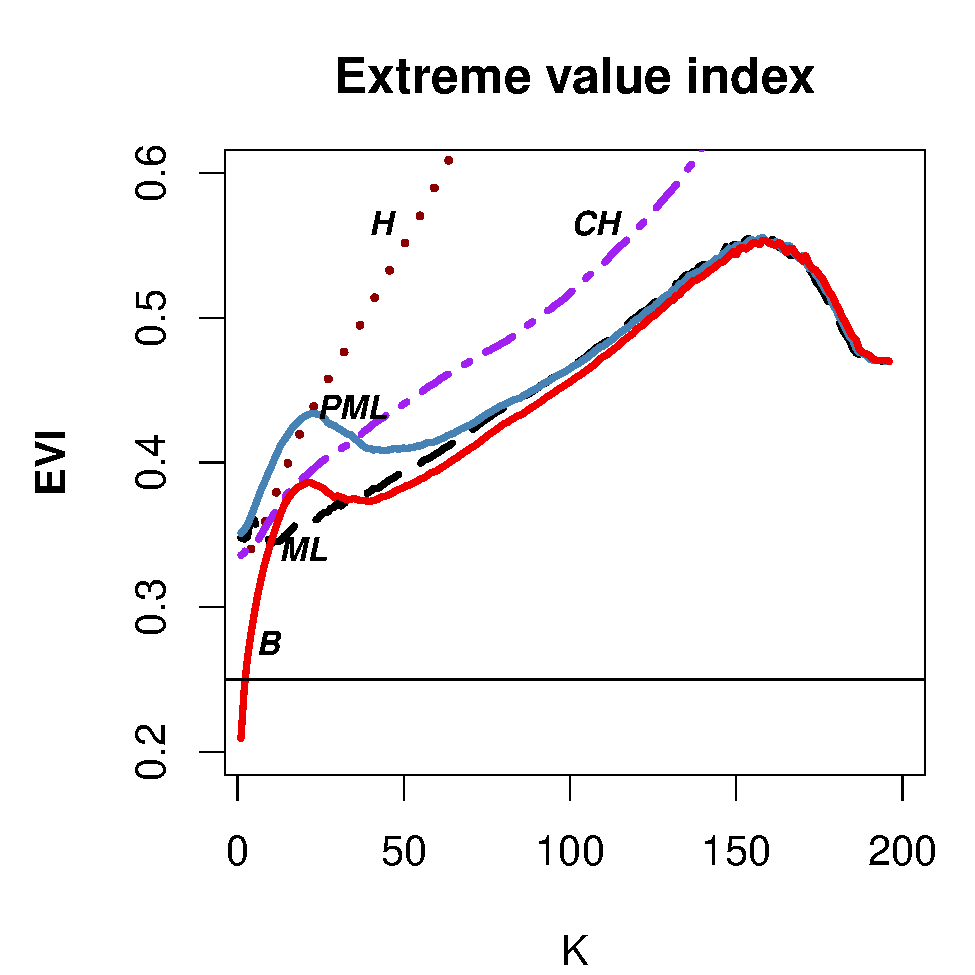
\includegraphics[width=\textwidth]{./plots/paper1/EVI_OutputGEV0,25200.pdf}
		\end{subfigure}
		\hspace{\fill}
		\begin{subfigure}[h]{0.40\linewidth}
			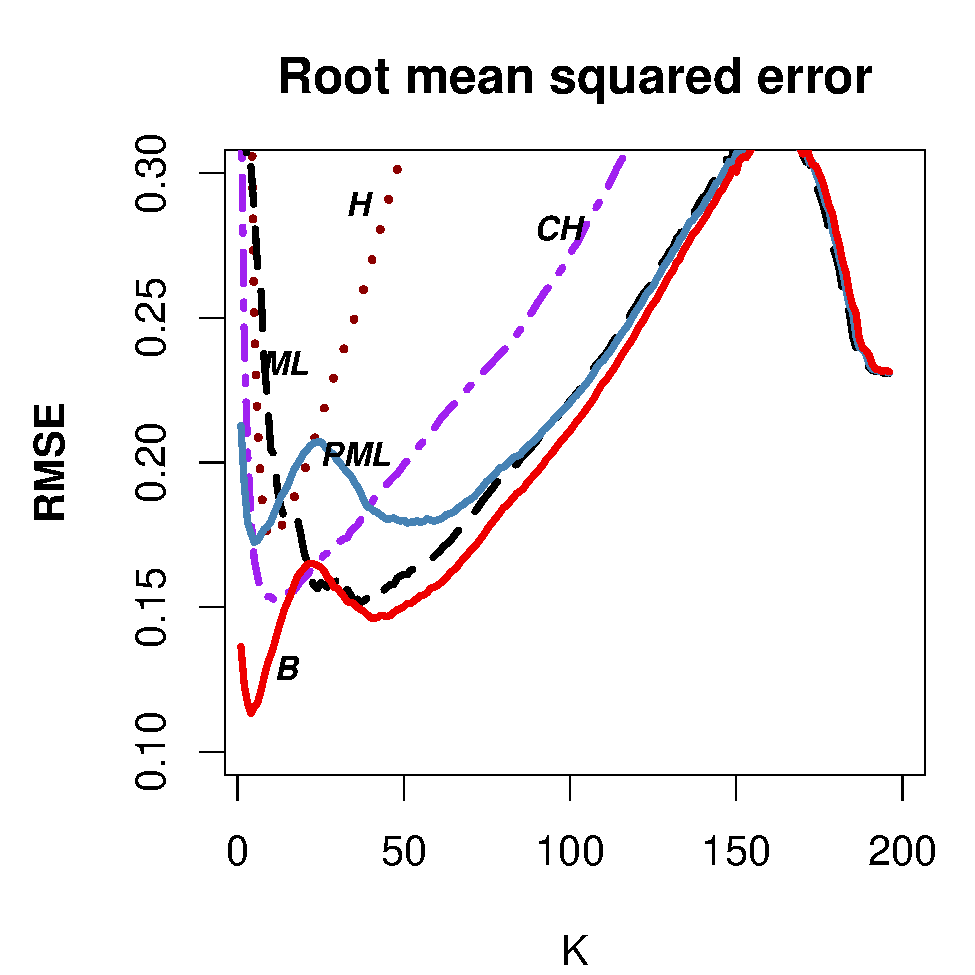
\includegraphics[width=\textwidth]{./plots/paper1/RMSE_OutputGEV0,25200.pdf}
		\end{subfigure}
		\bigskip
		\centering
		\begin{subfigure}[h]{0.40\linewidth}
			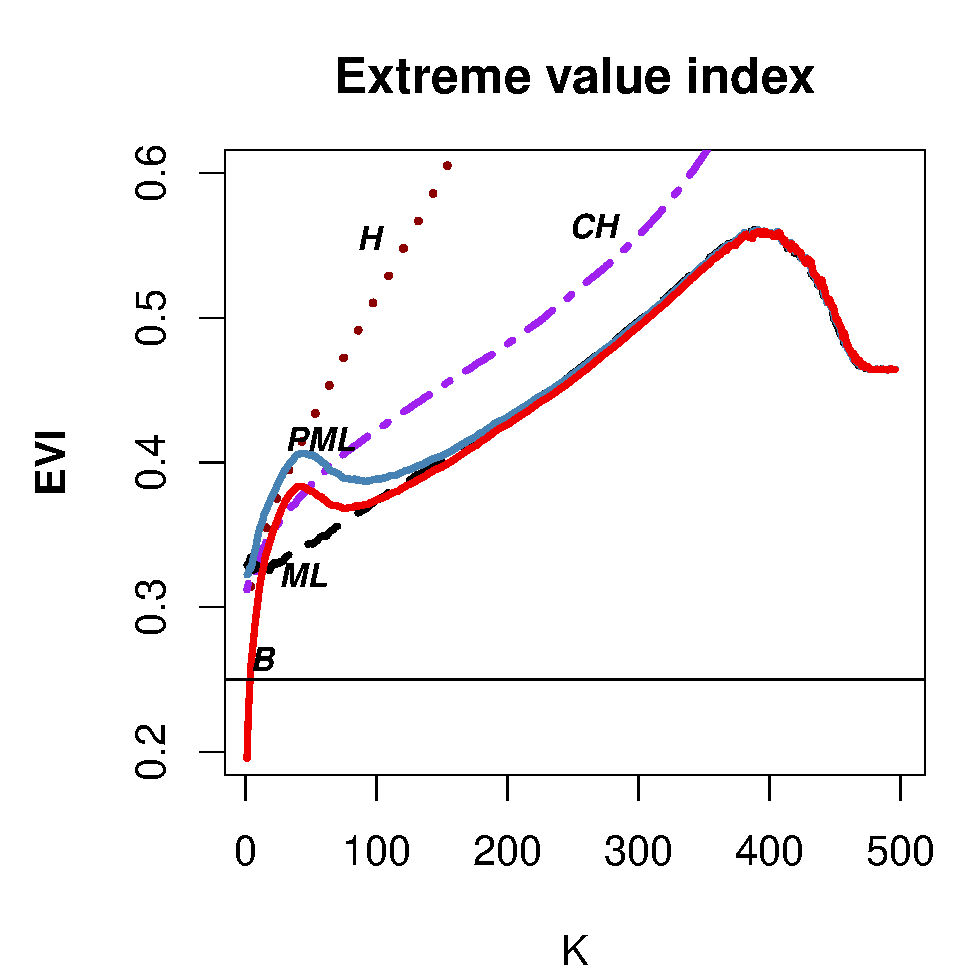
\includegraphics[width=\textwidth]{./plots/paper1/EVI_OutputGEV0,25500.pdf}
		\end{subfigure}
		\hspace{\fill}
		\begin{subfigure}[h]{0.40\linewidth}
			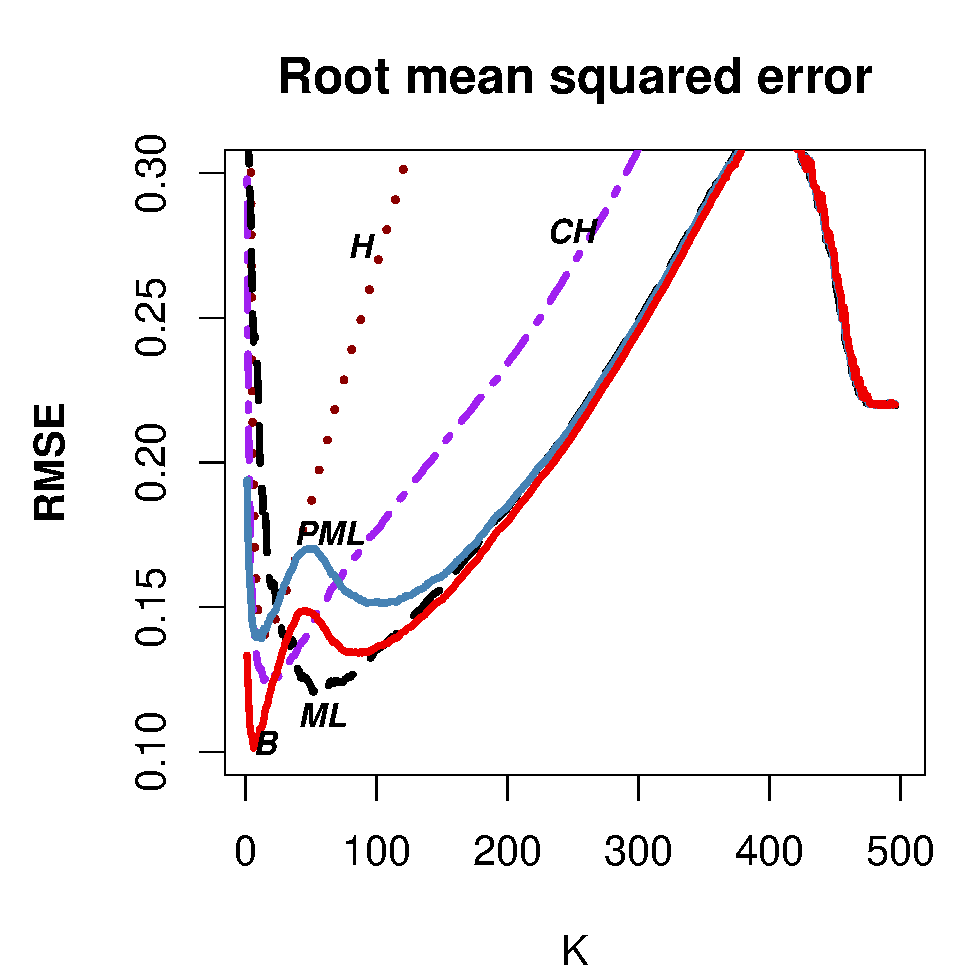
\includegraphics[width=\textwidth]{./plots/paper1/RMSE_OutputGEV0,25500.pdf}
		\end{subfigure}
		\bigskip
		\centering
		\begin{subfigure}[h]{0.40\linewidth}
			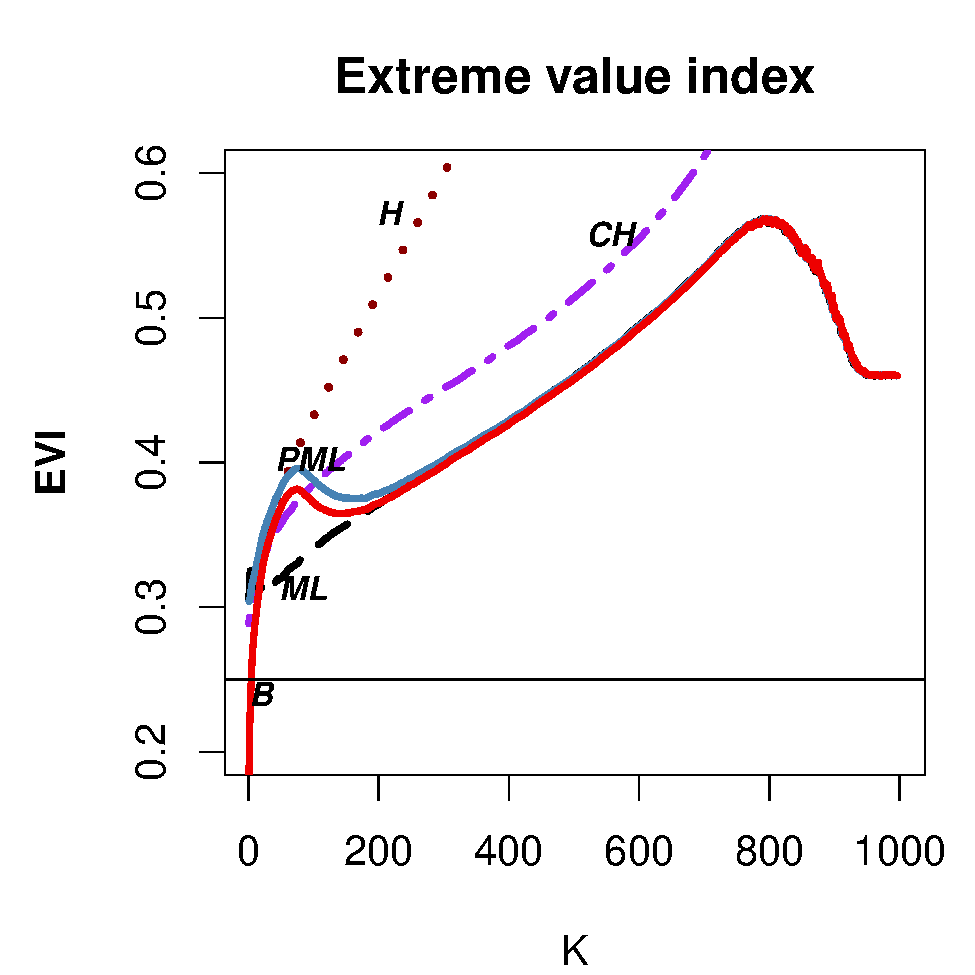
\includegraphics[width=\textwidth]{./plots/paper1/EVI_OutputGEV0,251000.pdf}
		\end{subfigure}
		\hspace{\fill}
		\begin{subfigure}[h]{0.40\linewidth}
			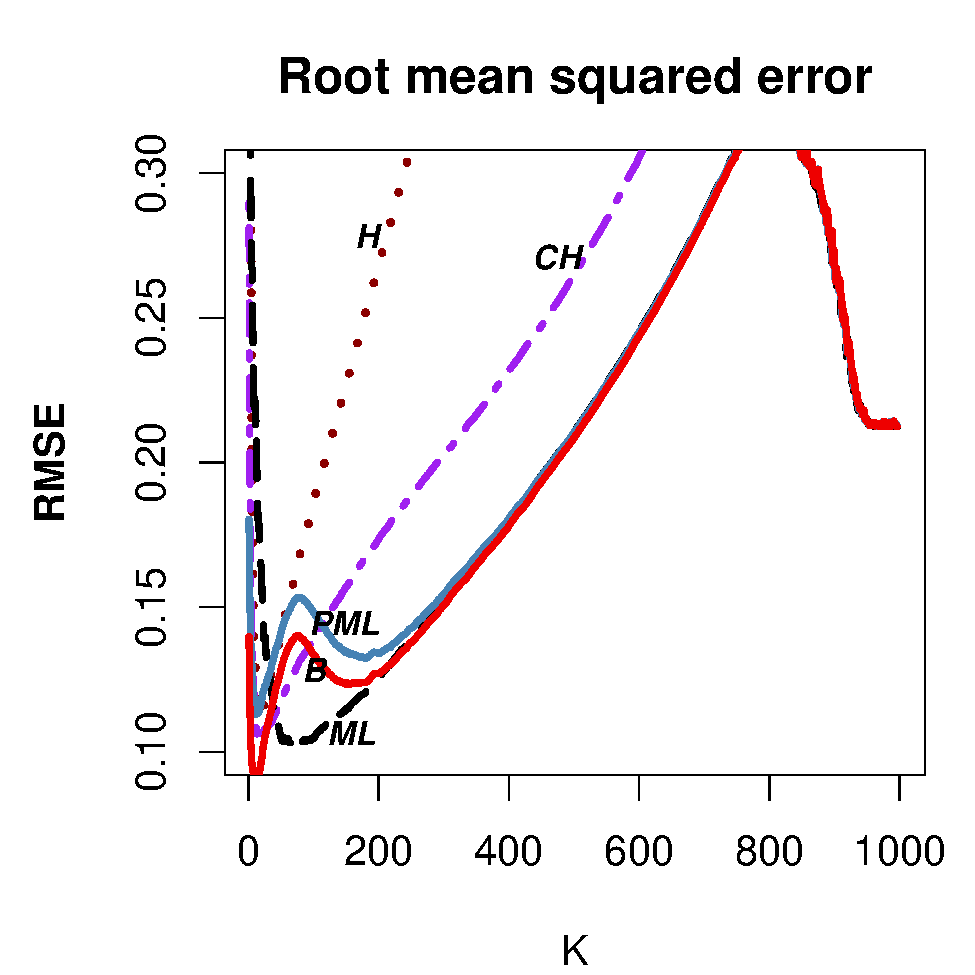
\includegraphics[width=\textwidth]{./plots/paper1/RMSE_OutputGEV0,251000.pdf}
		\end{subfigure}
	\caption{Bias (left) and root mean squared error (right) in case of the \textbf{EV distribution} with $\gamma=0.25$ for sample sizes $n=200$ (top), $n=500$ (middle) and $n=1000$ (bottom) for the Hill estimator (H), the EPD-ML estimator $\hat{\gamma}_{k}^{ML}$ (ML), the penalised ML estimator $\hat{\gamma}^P_{k}(1)$ with $\omega=1$ (PML), the Bayesian estimator $\hat{\gamma}^B_{k}(1)$ with $\omega=1$ (B), and the minimum variance reduced bias estimator $CH_k$ (CH).}
	\label{paper1:fig1}
\end{figure}
	\begin{figure}[h]
		\centering
		\begin{subfigure}[h]{0.40\linewidth}
			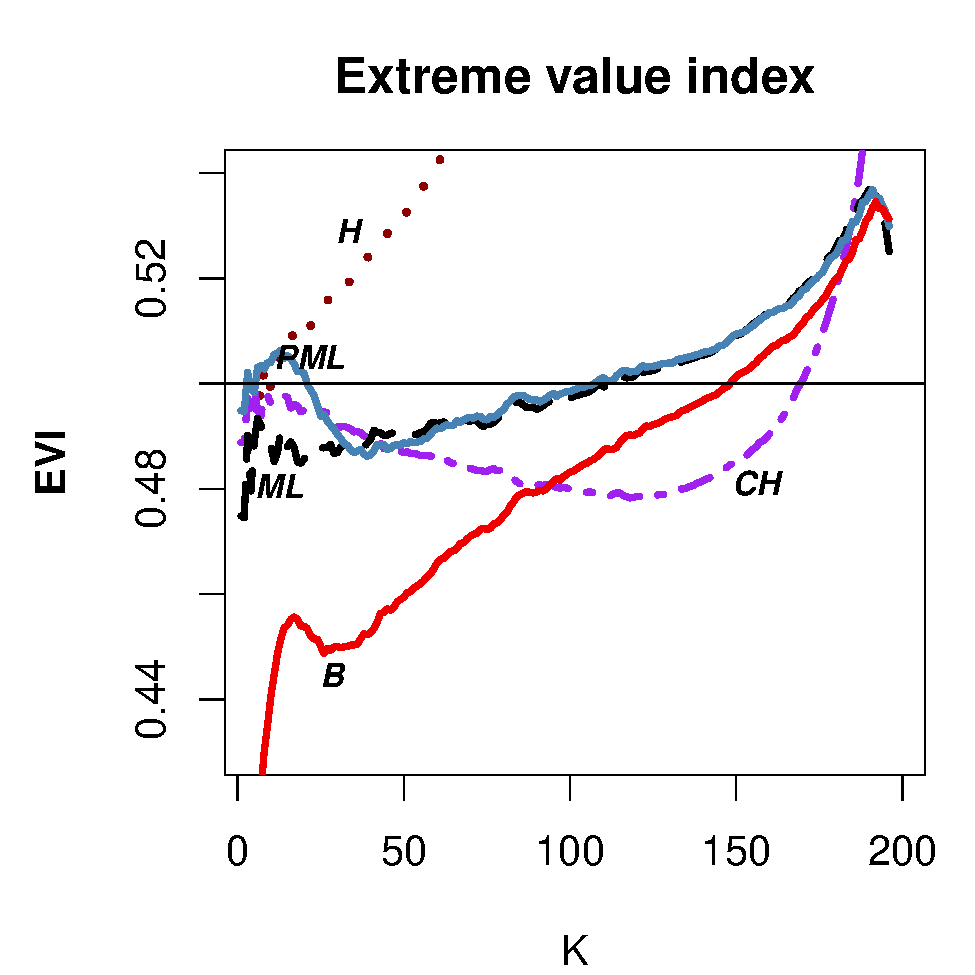
\includegraphics[width=\textwidth]{./plots/paper1/EVI_Outputfrehet0,5200.pdf}
		\end{subfigure}
		\hspace{\fill}
		\begin{subfigure}[h]{0.40\linewidth}
			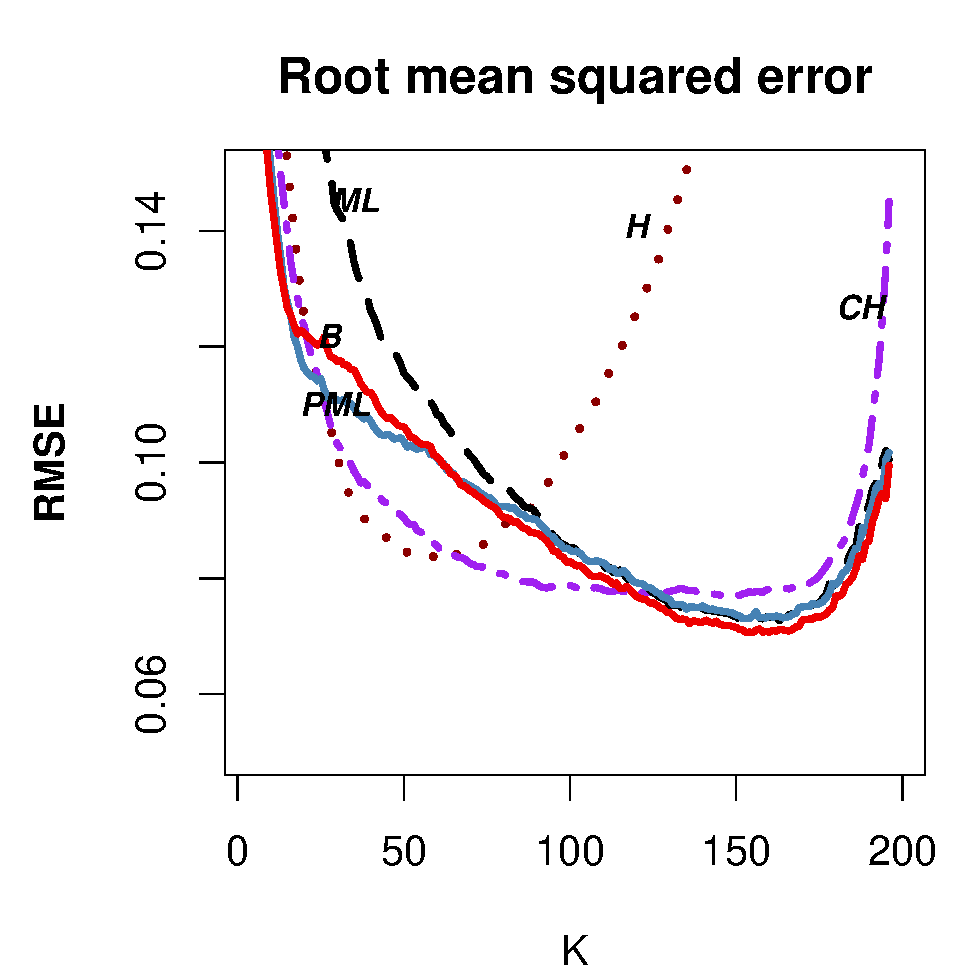
\includegraphics[width=\textwidth]{./plots/paper1/RMSE_Outputfrehet0,5200.pdf}
		\end{subfigure}
		\bigskip
		\centering
		\begin{subfigure}[h]{0.40\linewidth}
			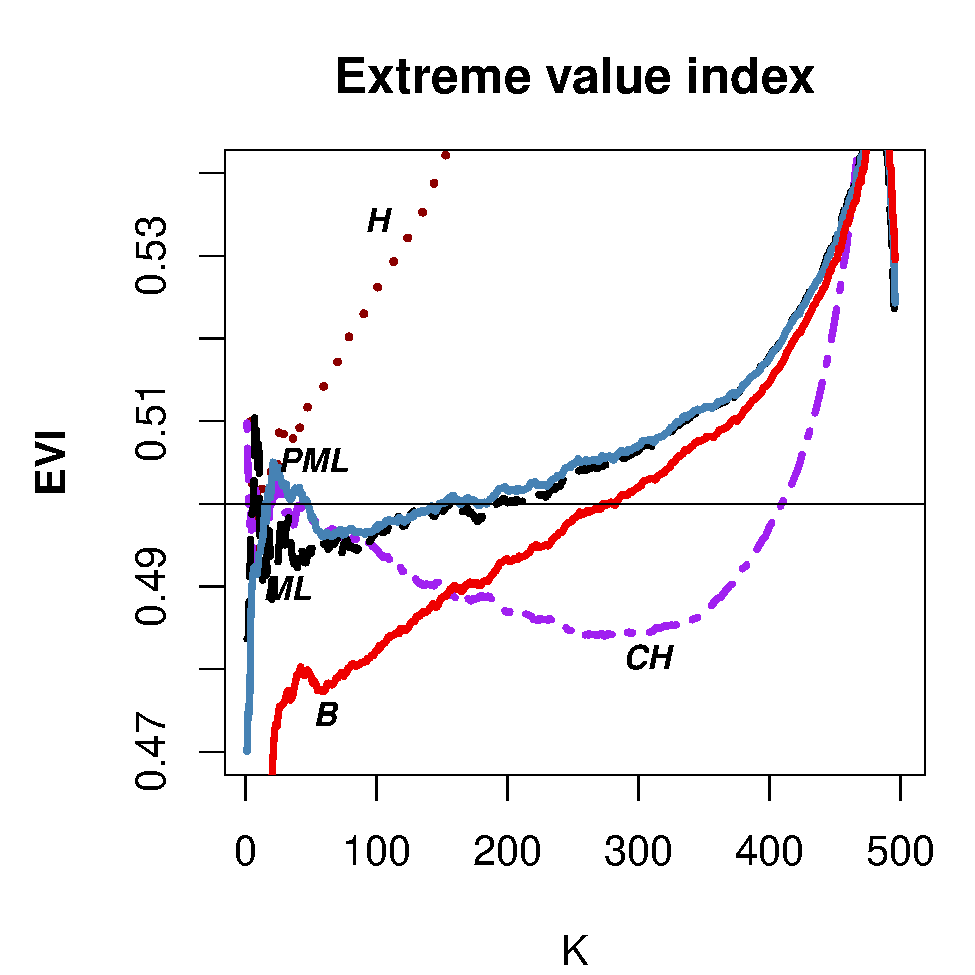
\includegraphics[width=\textwidth]{./plots/paper1/EVI_Outputfrehet0,5500.pdf}
		\end{subfigure}
		\hspace{\fill}
		\begin{subfigure}[h]{0.40\linewidth}
			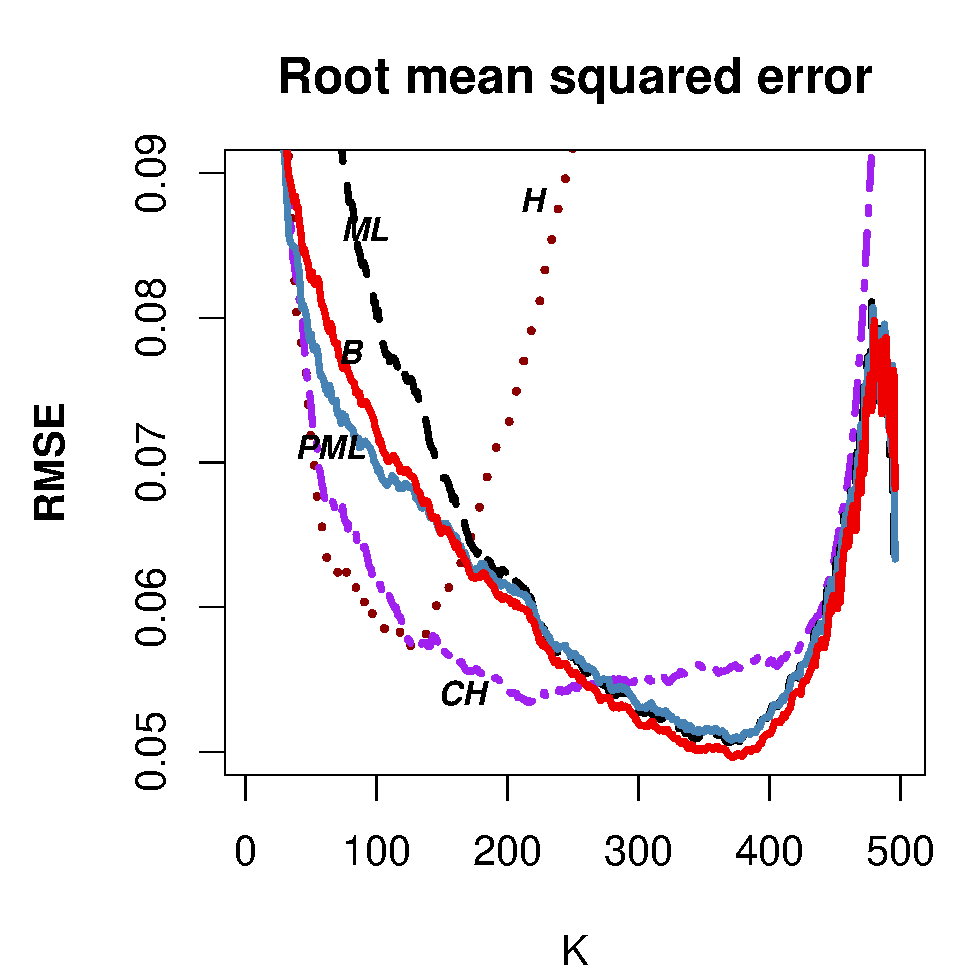
\includegraphics[width=\textwidth]{./plots/paper1/RMSE_Outputfrehet0,5500.pdf}
		\end{subfigure}
		\bigskip
		\centering
		\begin{subfigure}[h]{0.40\linewidth}
			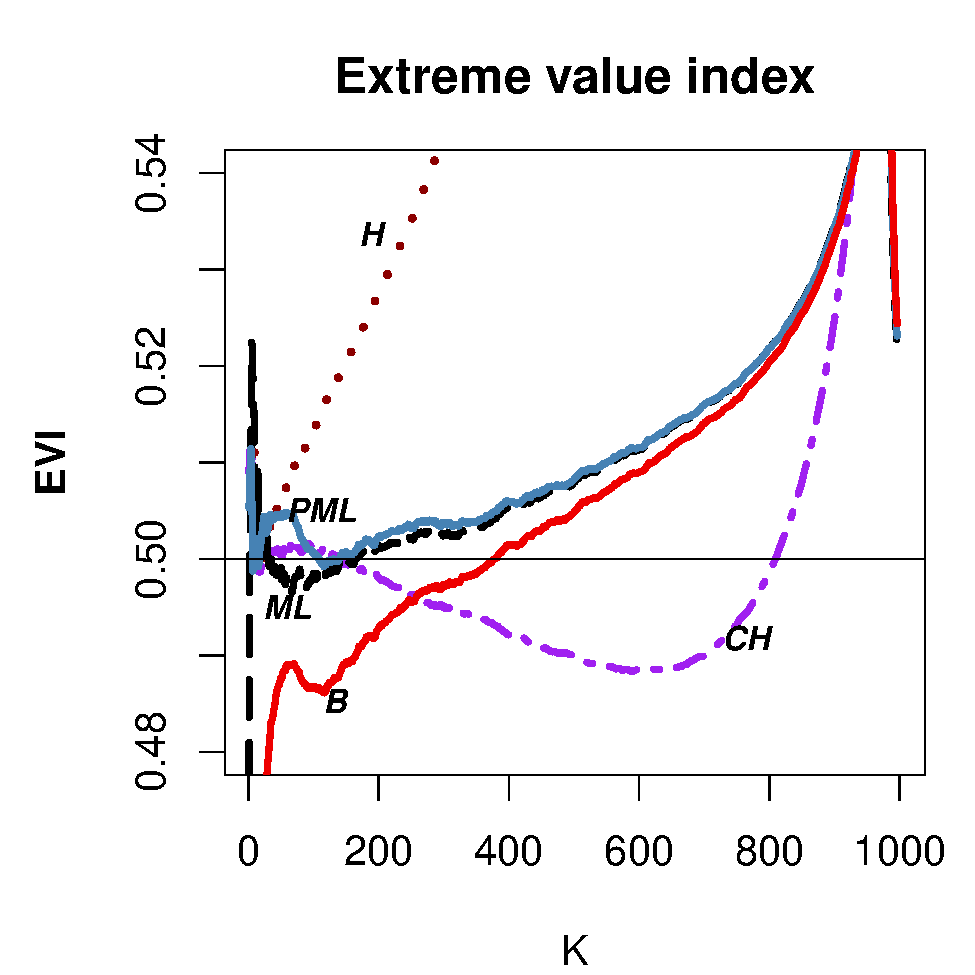
\includegraphics[width=\textwidth]{./plots/paper1/EVI_Outputfrehet0,51000.pdf}
		\end{subfigure}
		\hspace{\fill}
		\begin{subfigure}[h]{0.40\linewidth}
			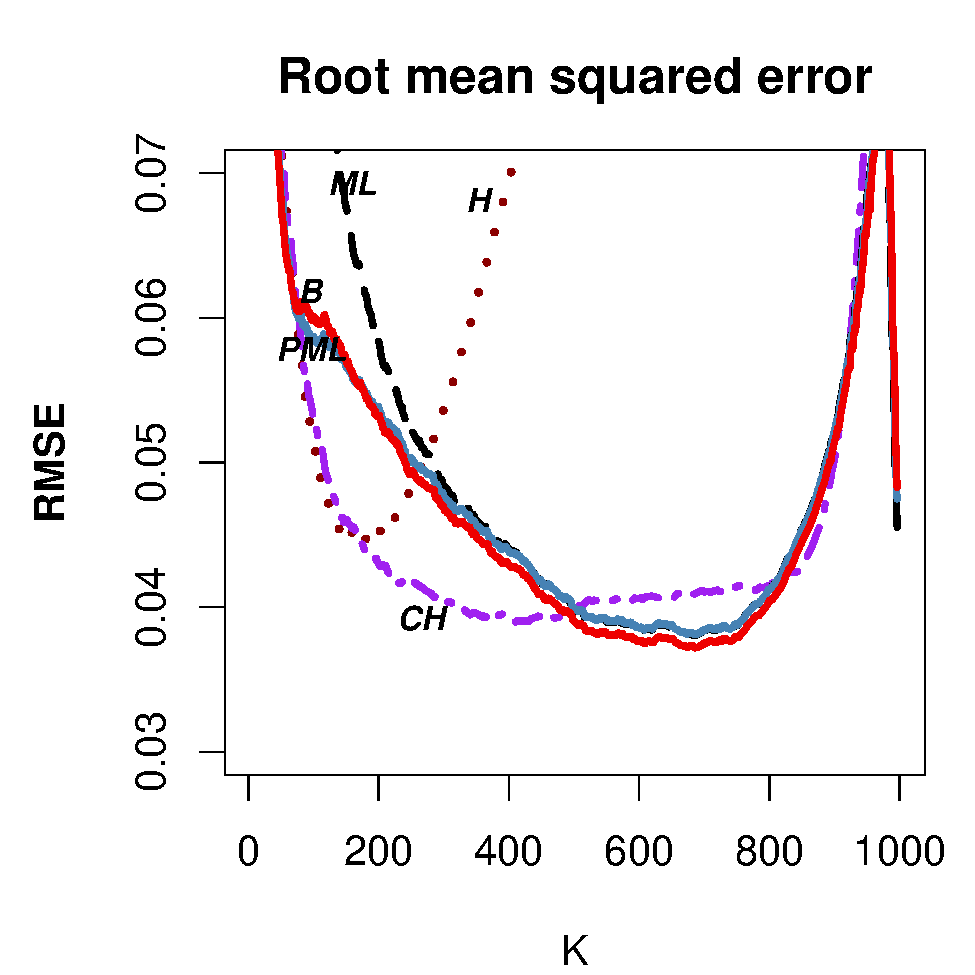
\includegraphics[width=\textwidth]{./plots/paper1/RMSE_Outputfrehet0,51000.pdf}
		\end{subfigure}
		\caption{Bias (left) and root mean squared error (right) in case of the \textbf{Fr\'echet distribution} with $\gamma=0.5$ for sample sizes $n=200$ (top), $n=500$ (middle) and $n=1000$ (bottom) for the Hill estimator (H), the EPD-ML estimator $\hat{\gamma}_{k}^{ML}$ (ML), the penalised ML estimator $\hat{\gamma}^P_{k}(1)$ with $\omega=1$ (PML), the Bayesian estimator $\hat{\gamma}^B_{k}(1)$ with $\omega=1$ (B), and the minimum variance reduced bias estimator $CH_k$ (CH).}
		\label{paper1:fig2}
	\end{figure}
	\begin{figure}[h]
		\centering
		\begin{subfigure}[h]{0.40\linewidth}
			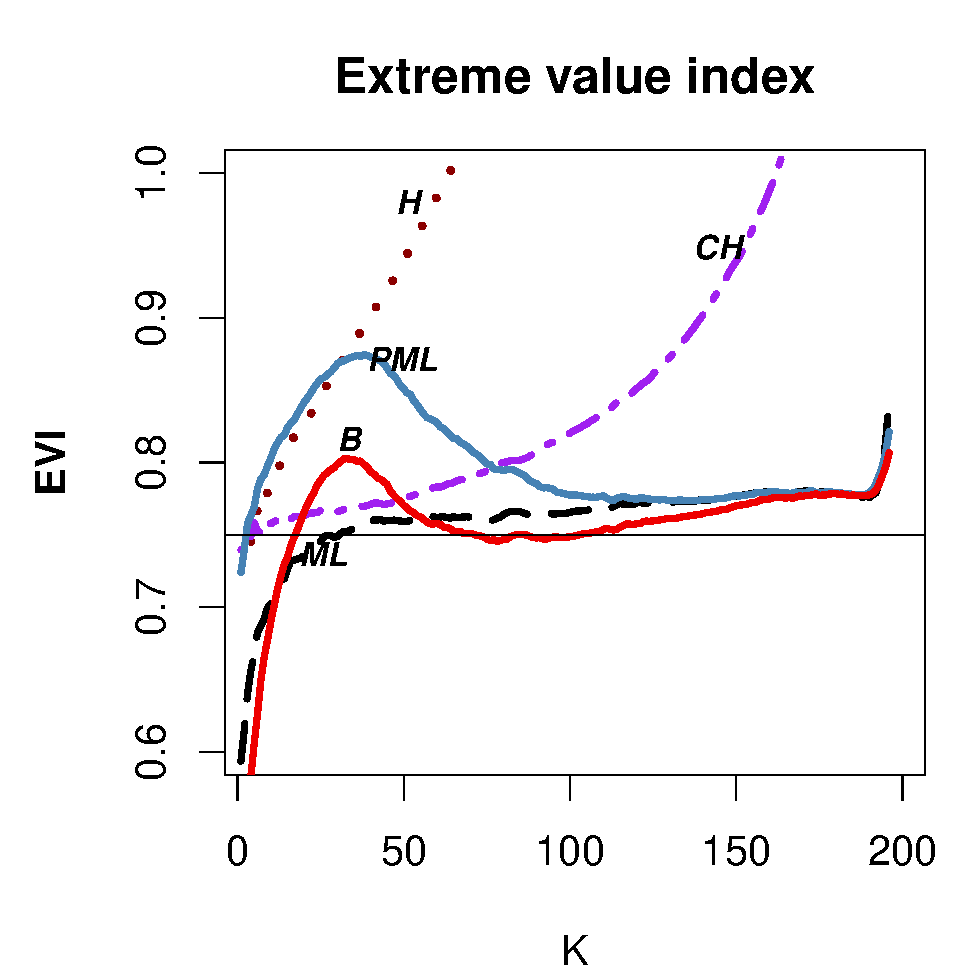
\includegraphics[width=\textwidth]{./plots/paper1/EVI_Outputburr0,75200.pdf}
		\end{subfigure}
		\hspace{\fill}
		\begin{subfigure}[h]{0.40\linewidth}
			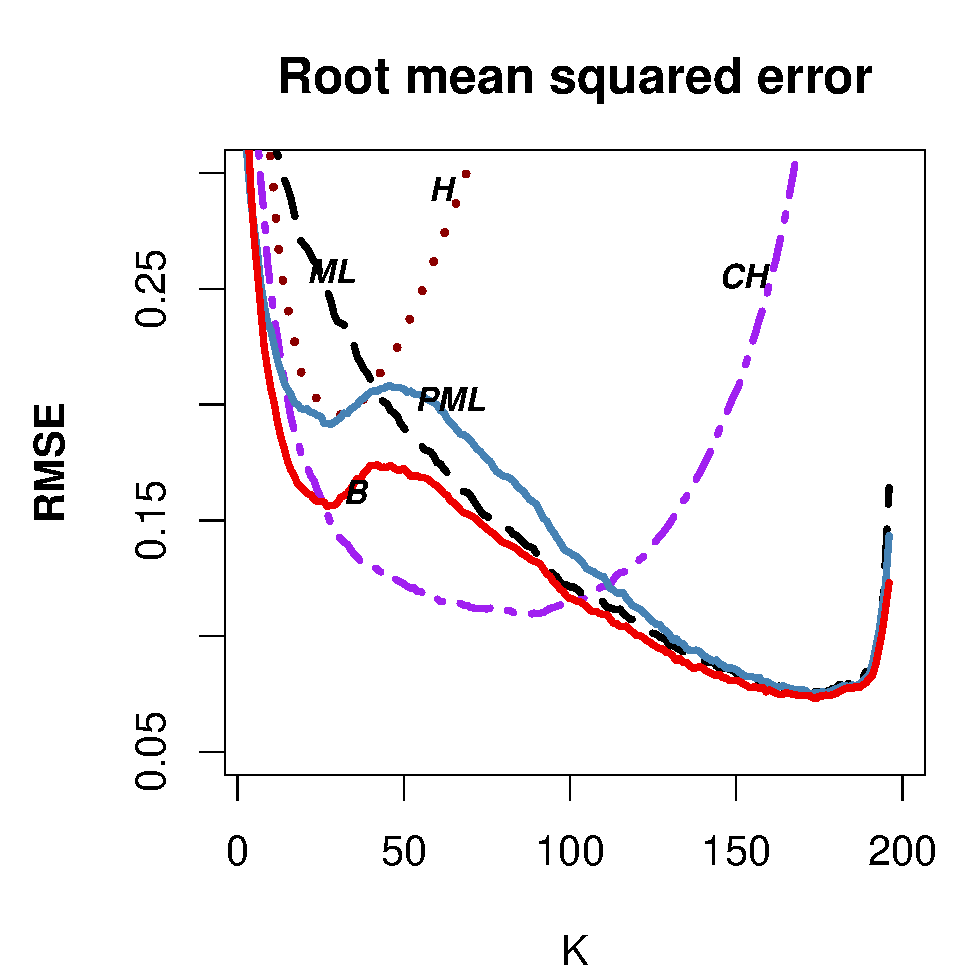
\includegraphics[width=\textwidth]{./plots/paper1/RMSE_Outputburr0,75200.pdf}
		\end{subfigure}
		\bigskip
		\centering
		\begin{subfigure}[h]{0.40\linewidth}
			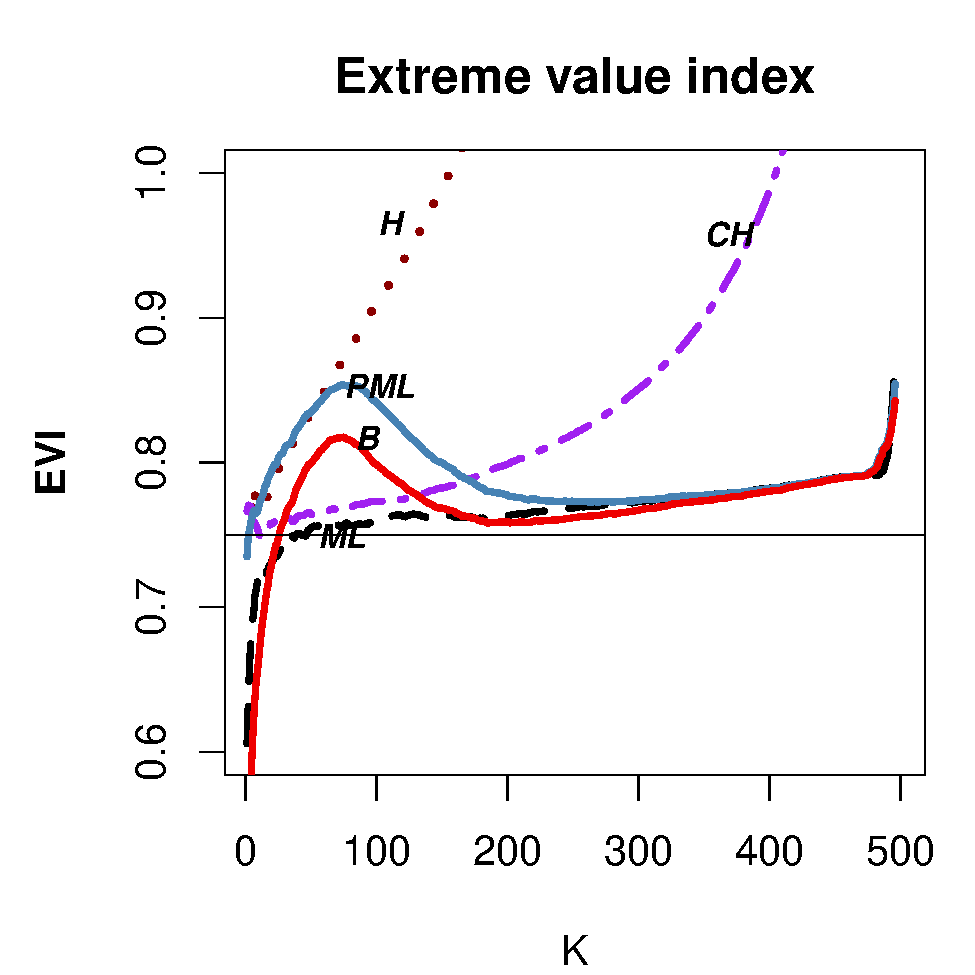
\includegraphics[width=\textwidth]{./plots/paper1/EVI_Outputburr0,75500.pdf}
		\end{subfigure}
		\hspace{\fill}
		\begin{subfigure}[h]{0.40\linewidth}
			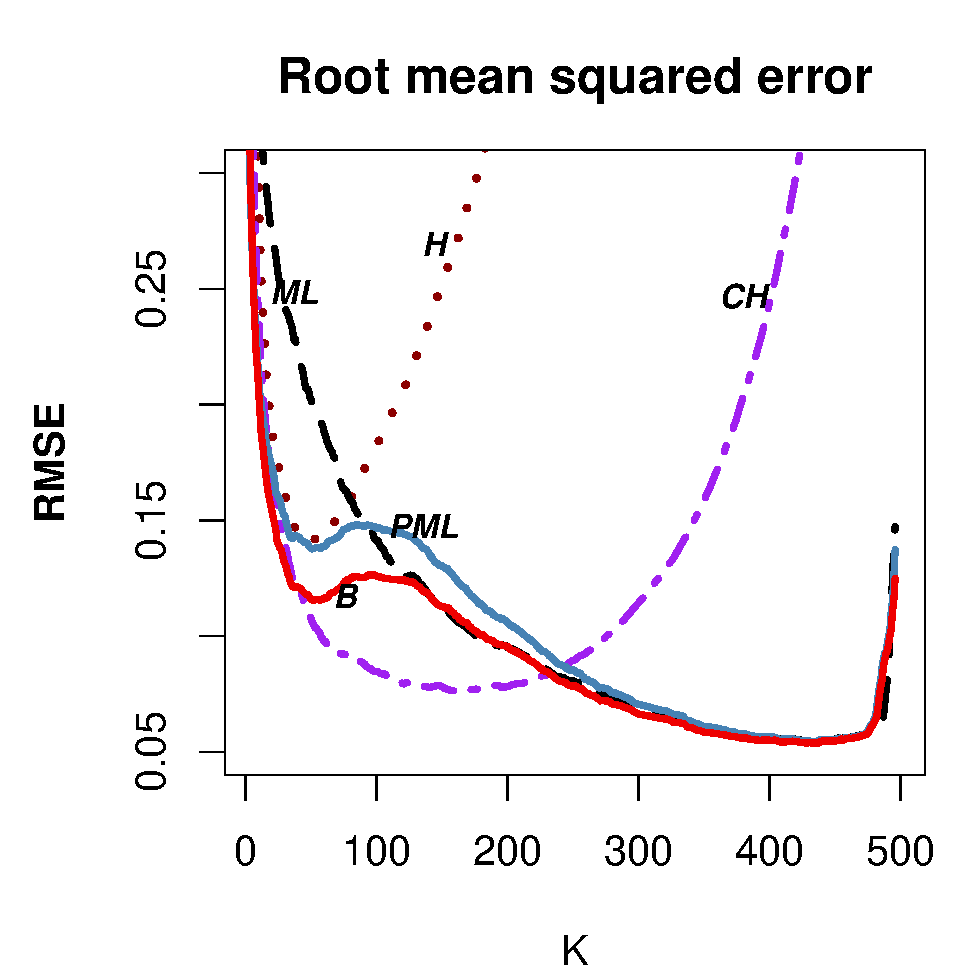
\includegraphics[width=\textwidth]{./plots/paper1/RMSE_Outputburr0,75500.pdf}
		\end{subfigure}
		\bigskip
		\centering
		\begin{subfigure}[h]{0.40\linewidth}
			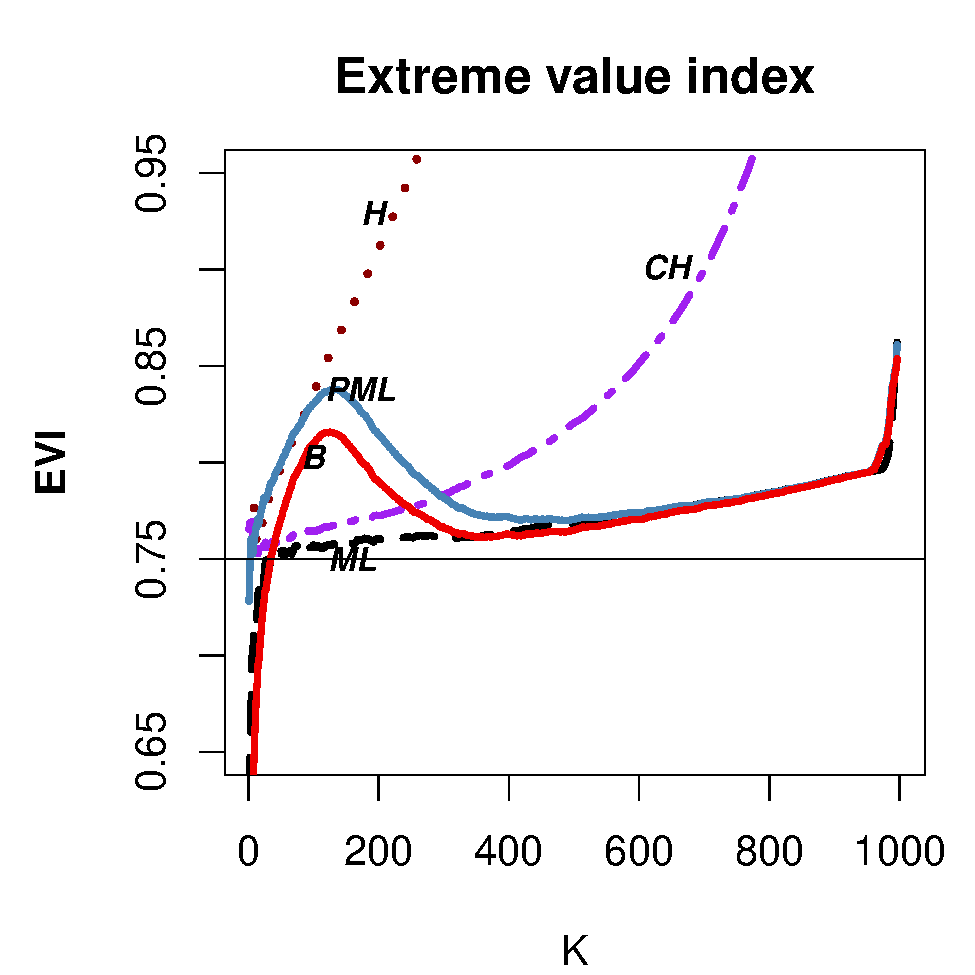
\includegraphics[width=\textwidth]{./plots/paper1/EVI_Outputburr0,751000.pdf}
		\end{subfigure}
		\hspace{\fill}
		\begin{subfigure}[h]{0.40\linewidth}
			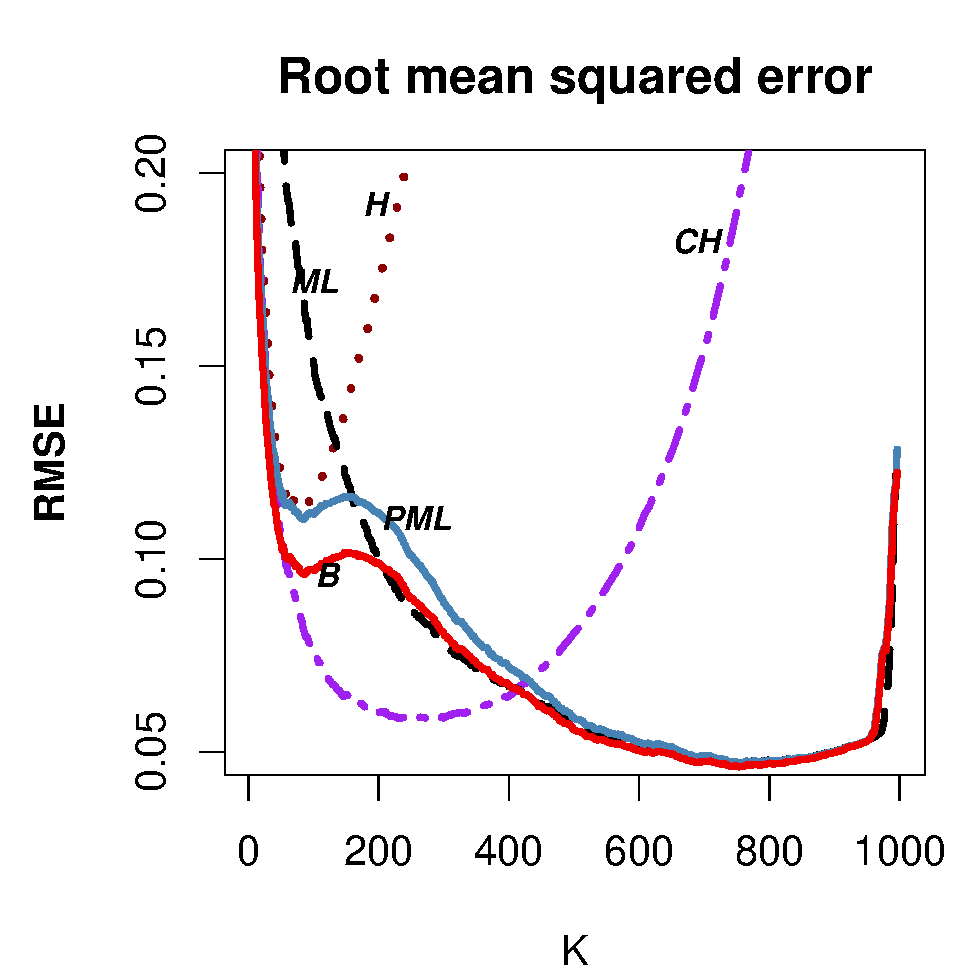
\includegraphics[width=\textwidth]{./plots/paper1/RMSE_Outputburr0,751000.pdf}
		\end{subfigure}
		\caption{Bias (left) and root mean squared error (right) in case of the \textbf{Burr distribution} with $\gamma=0.75$ for sample sizes $n=200$ (top), $n=500$ (middle) and $n=1000$ (bottom) for the Hill estimator (H), the EPD-ML estimator $\hat{\gamma}_{k}^{ML}$ (ML), the penalised ML estimator $\hat{\gamma}^P_{k}(1)$ with $\omega=1$ (PML), the Bayesian estimator $\hat{\gamma}^B_{k}(1)$ with $\omega=1$ (B), and the minimum variance reduced bias estimator $CH_k$ (CH).}
		\label{paper1:fig3}
	\end{figure}
	\begin{figure}[h]
		\centering
		\begin{subfigure}[h]{0.40\linewidth}
			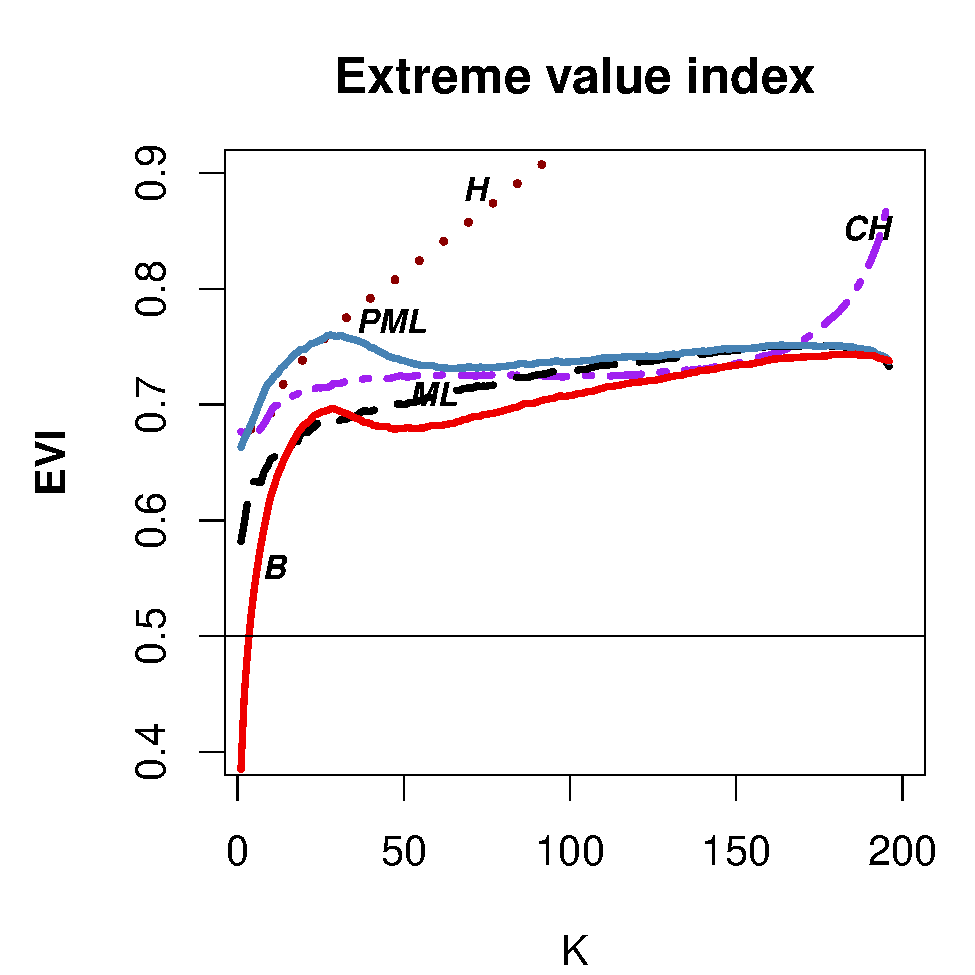
\includegraphics[width=\textwidth]{./plots/paper1/EVI_Outputloggamma0,5200.pdf}
		\end{subfigure}
	\hspace{\fill}
		\begin{subfigure}[h]{0.40\linewidth}
			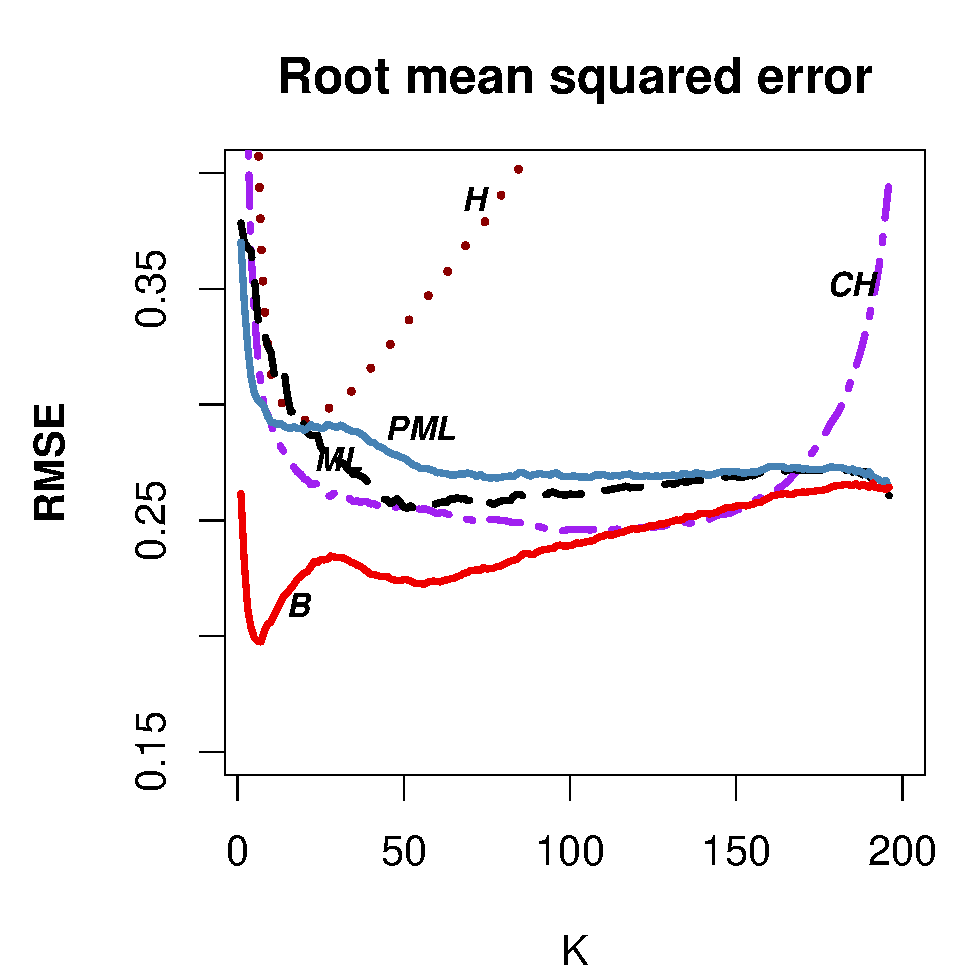
\includegraphics[width=\textwidth]{./plots/paper1/RMSE_Outputloggamma0,5200.pdf}
		\end{subfigure}
		\bigskip
		\centering
		\begin{subfigure}[h]{0.40\linewidth}
			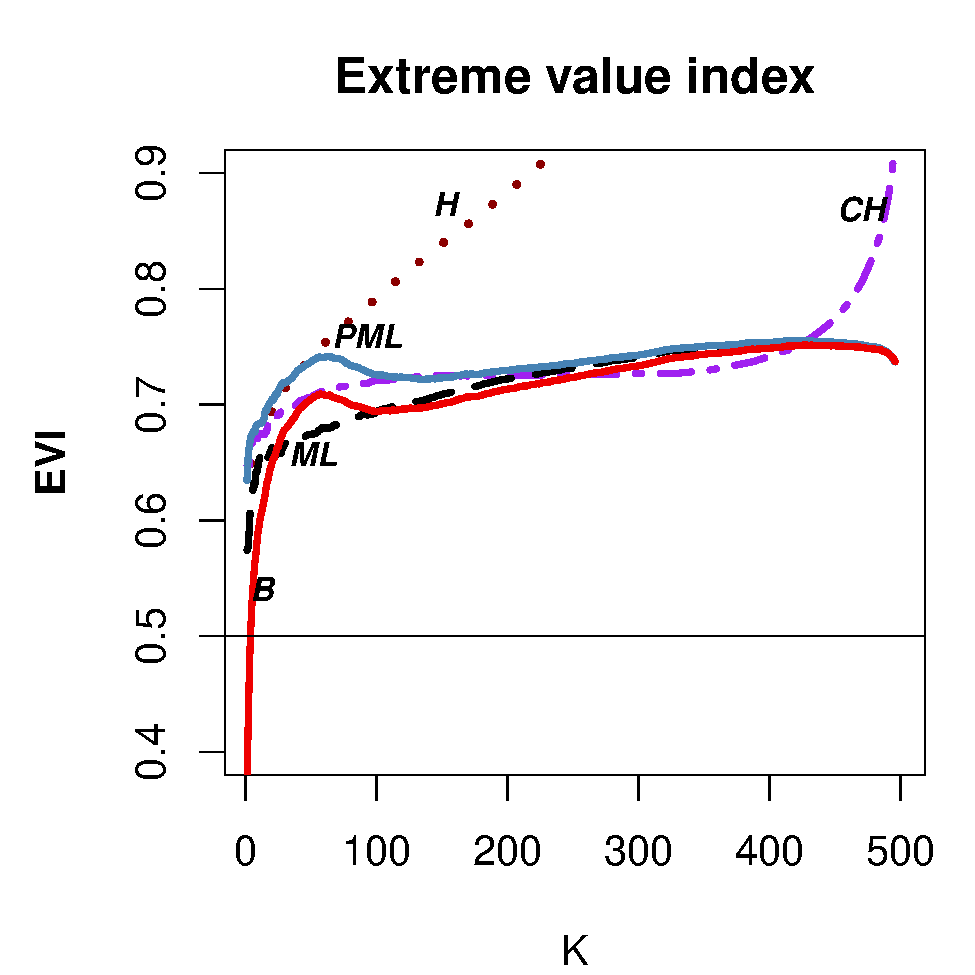
\includegraphics[width=\textwidth]{./plots/paper1/EVI_Outputloggamma0,5500.pdf}
		\end{subfigure}
		\hspace{\fill}
		\begin{subfigure}[h]{0.40\linewidth}
			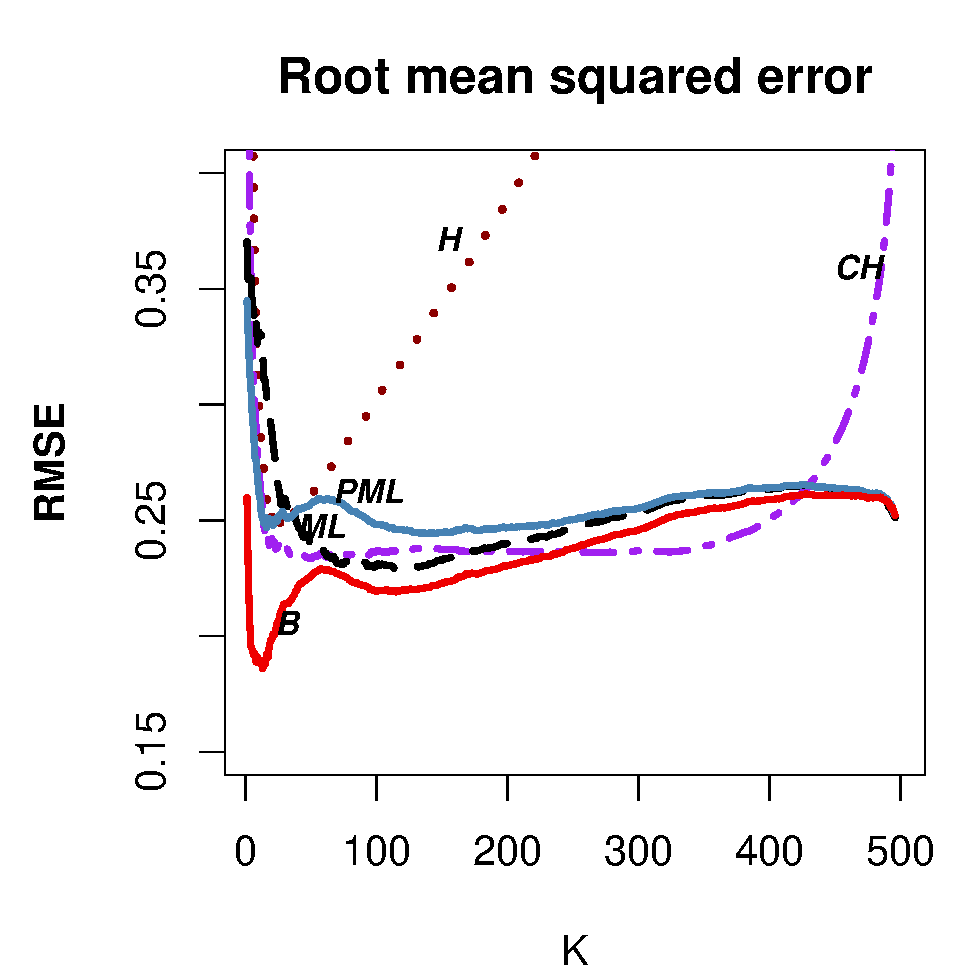
\includegraphics[width=\textwidth]{./plots/paper1/RMSE_Outputloggamma0,5500.pdf}
		\end{subfigure}
		\bigskip
		\centering
		\begin{subfigure}[h]{0.40\linewidth}
			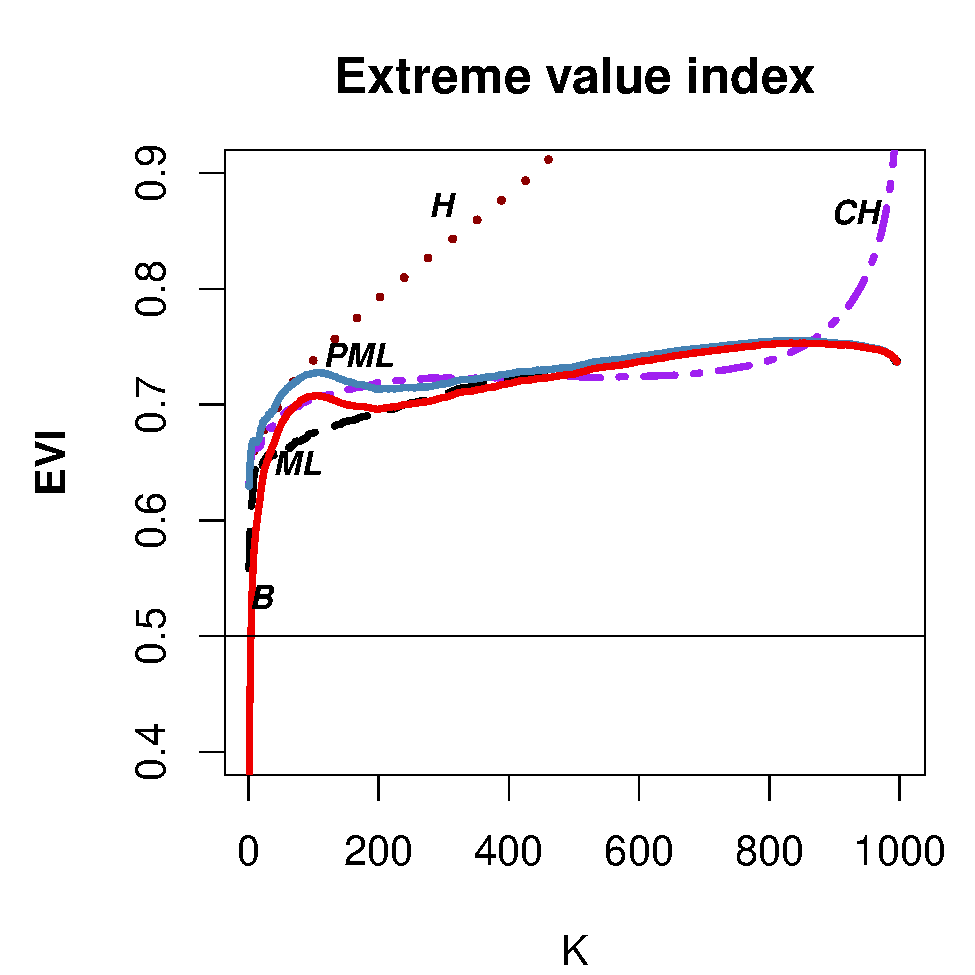
\includegraphics[width=\textwidth]{./plots/paper1/EVI_Outputloggamma0,51000.pdf}
		\end{subfigure}
		\hspace{\fill}
		\begin{subfigure}[h]{0.40\linewidth}
			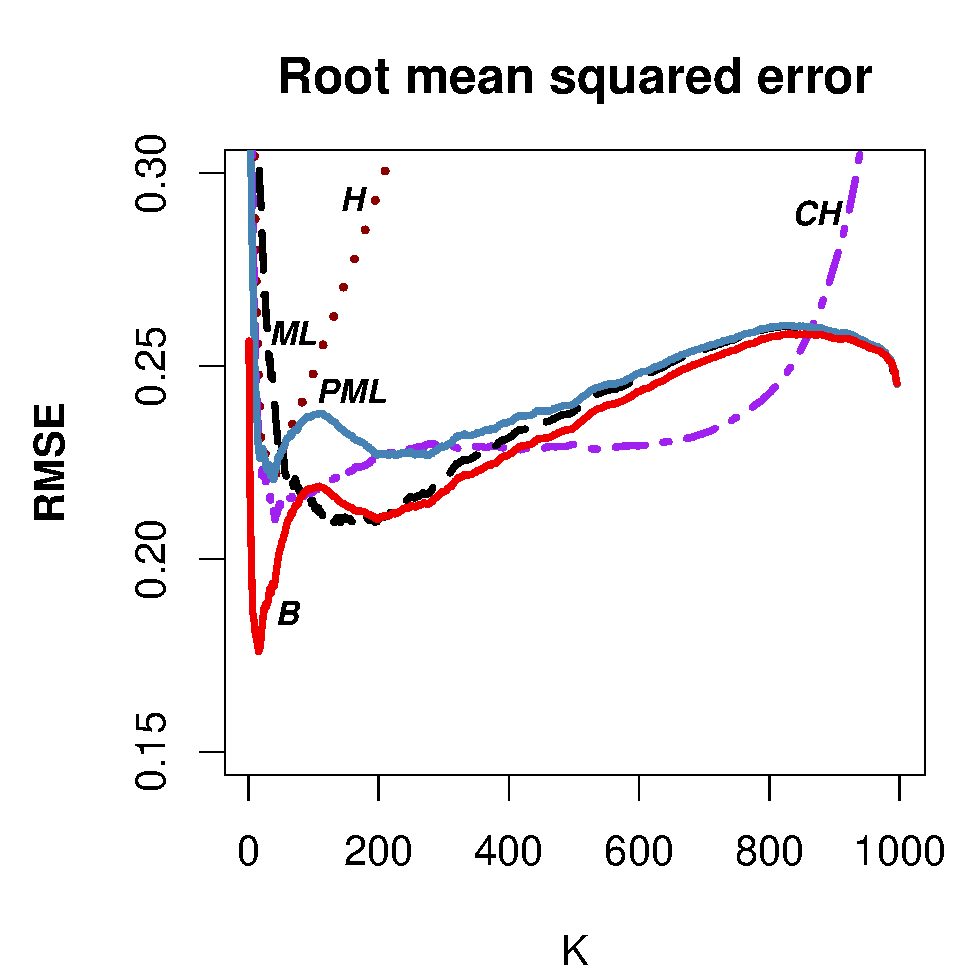
\includegraphics[width=\textwidth]{./plots/paper1/RMSE_Outputloggamma0,51000.pdf}
		\end{subfigure}
		\caption{Bias (left) and root mean squared error (right) in case of the \textbf{loggamma distribution} with $\gamma=0.5$ for sample sizes $n=200$ (top), $n=500$ (middle) and $n=1000$ (bottom) for the Hill estimator (H), the EPD-ML estimator $\hat{\gamma}_{k}^{ML}$ (ML), the penalised ML estimator $\hat{\gamma}^P_{k}(1)$ with $\omega=1$ (PML), the Bayesian estimator $\hat{\gamma}^B_{k}(1)$ with $\omega=1$ (B), and the minimum variance reduced bias estimator $CH_k$ (CH).}
		\label{paper1:fig4}
	\end{figure}
	\begin{figure}[h]
		\centering
		\begin{subfigure}[h]{0.40\linewidth}
			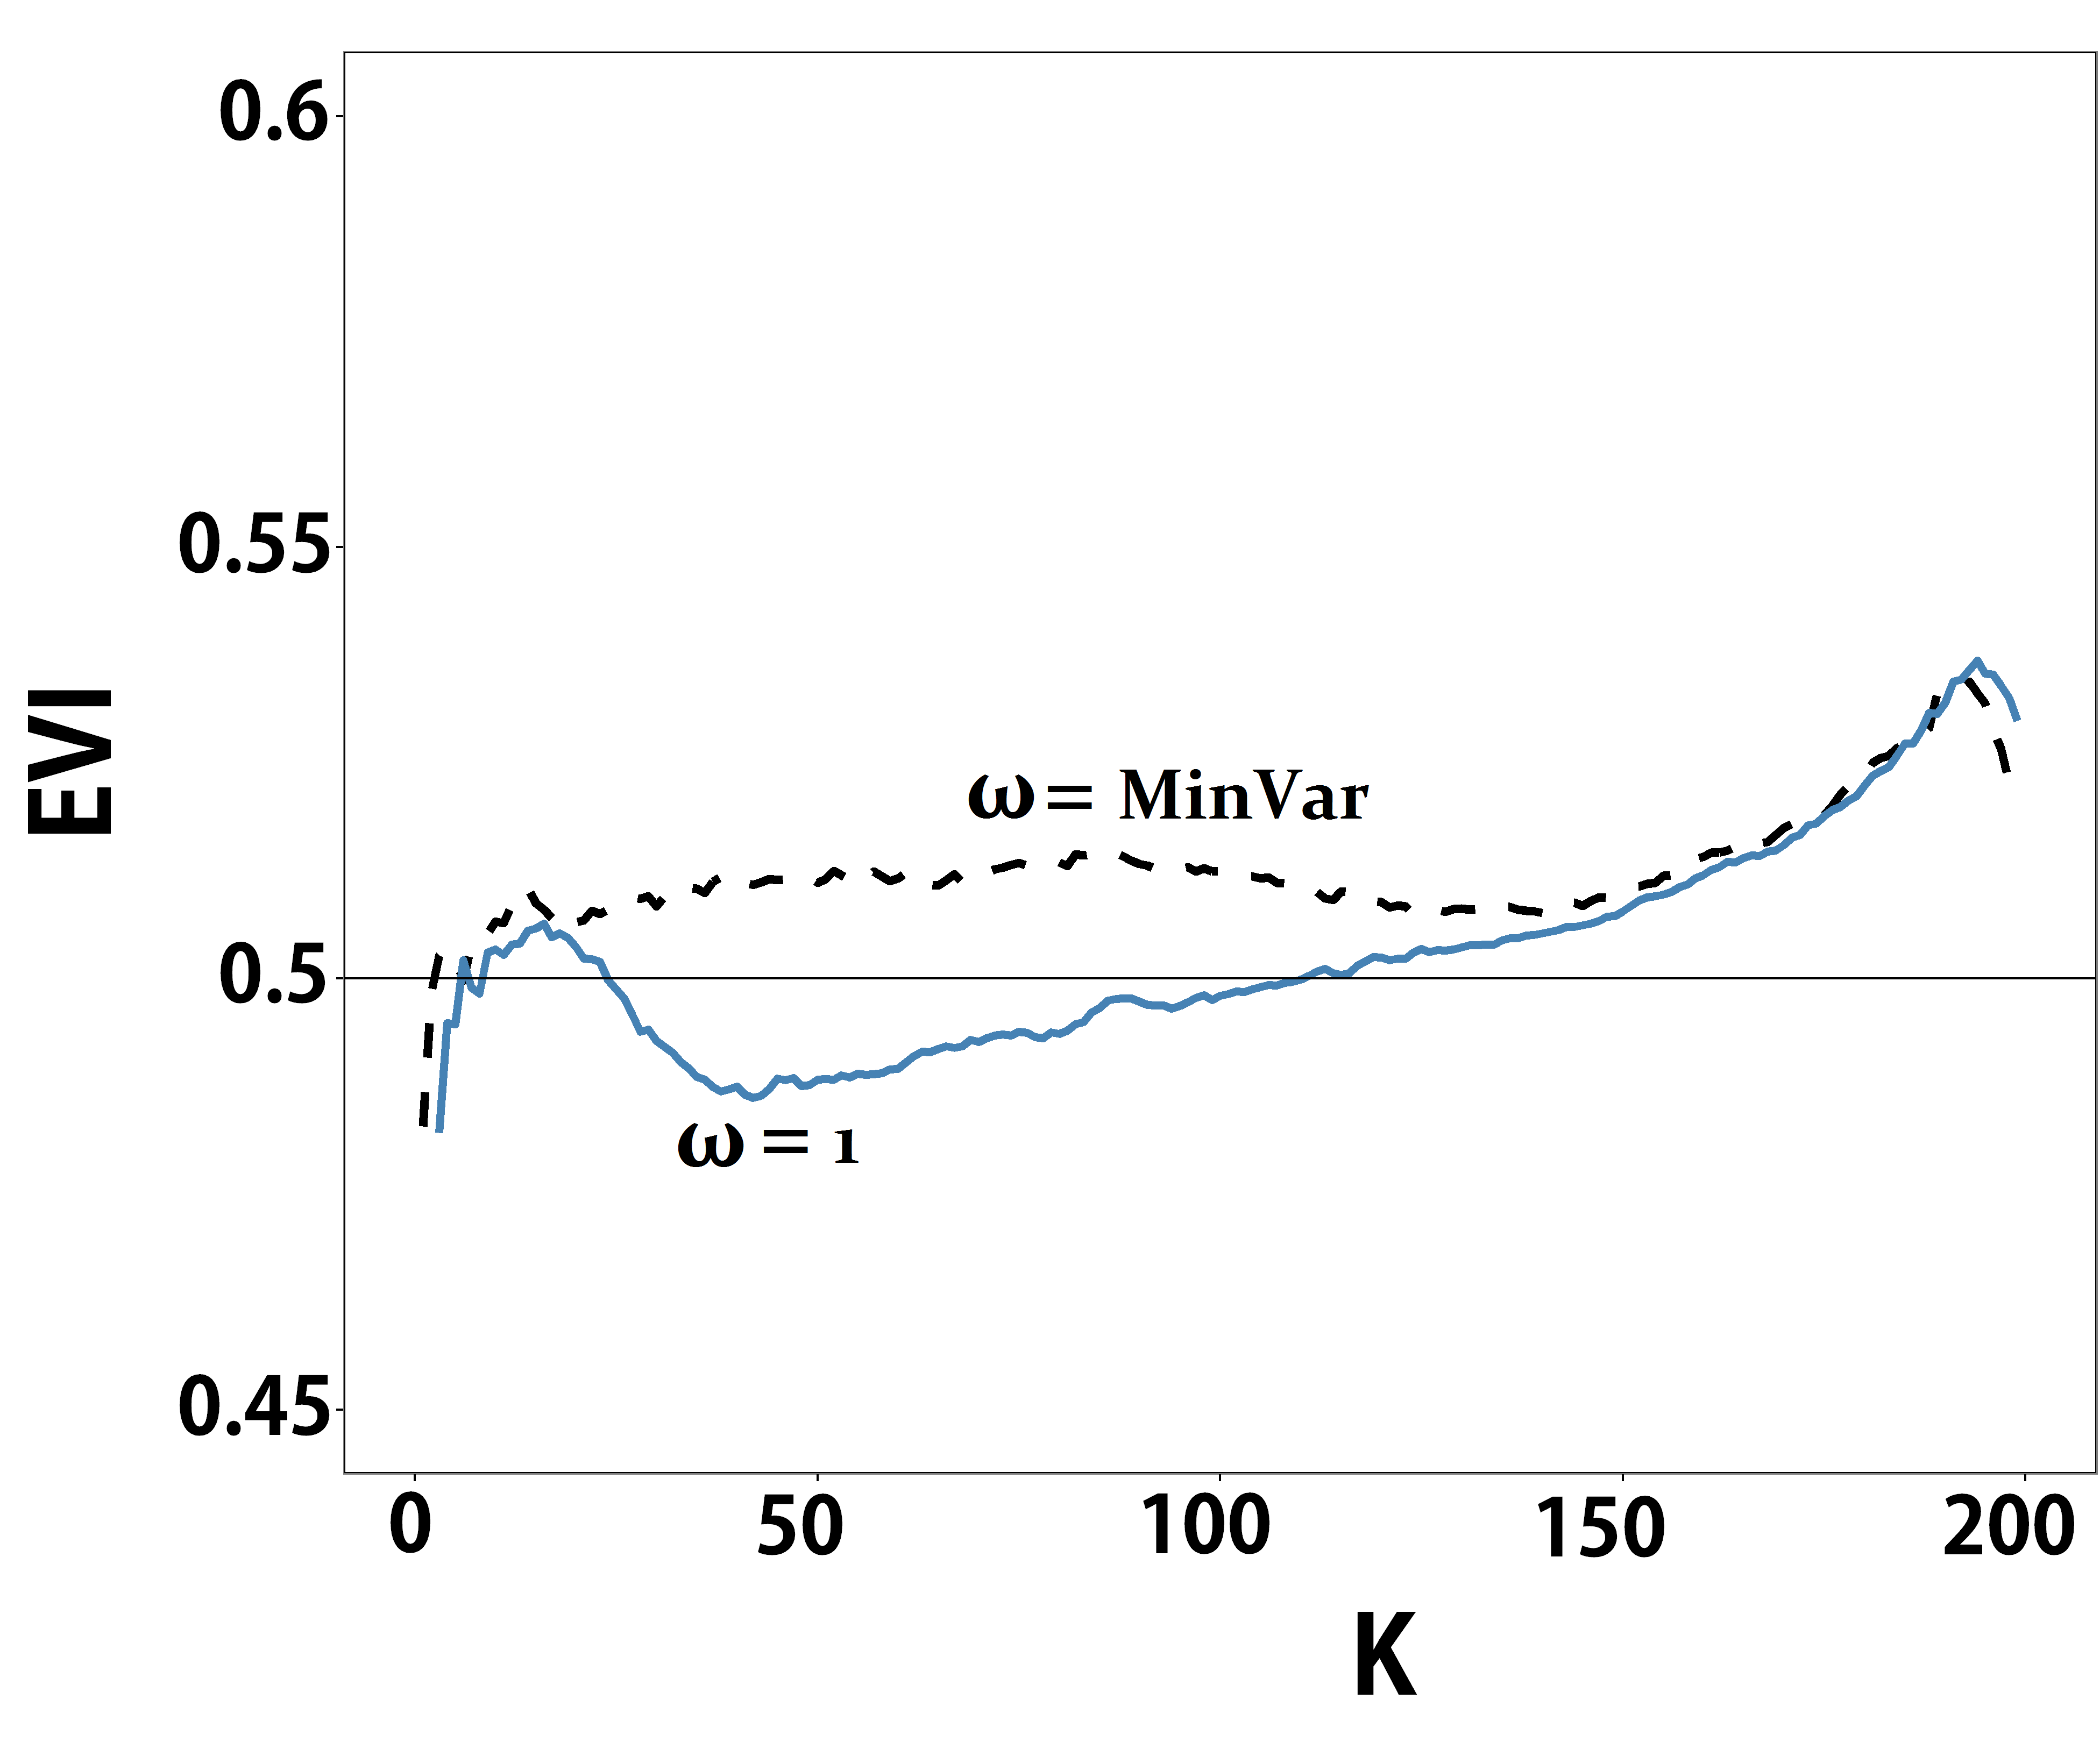
\includegraphics[width=65mm]{./plots/paper1/eviFrechetKappa.png}
		\end{subfigure}
		\hspace{\fill}
		\begin{subfigure}[h]{0.40\linewidth}
			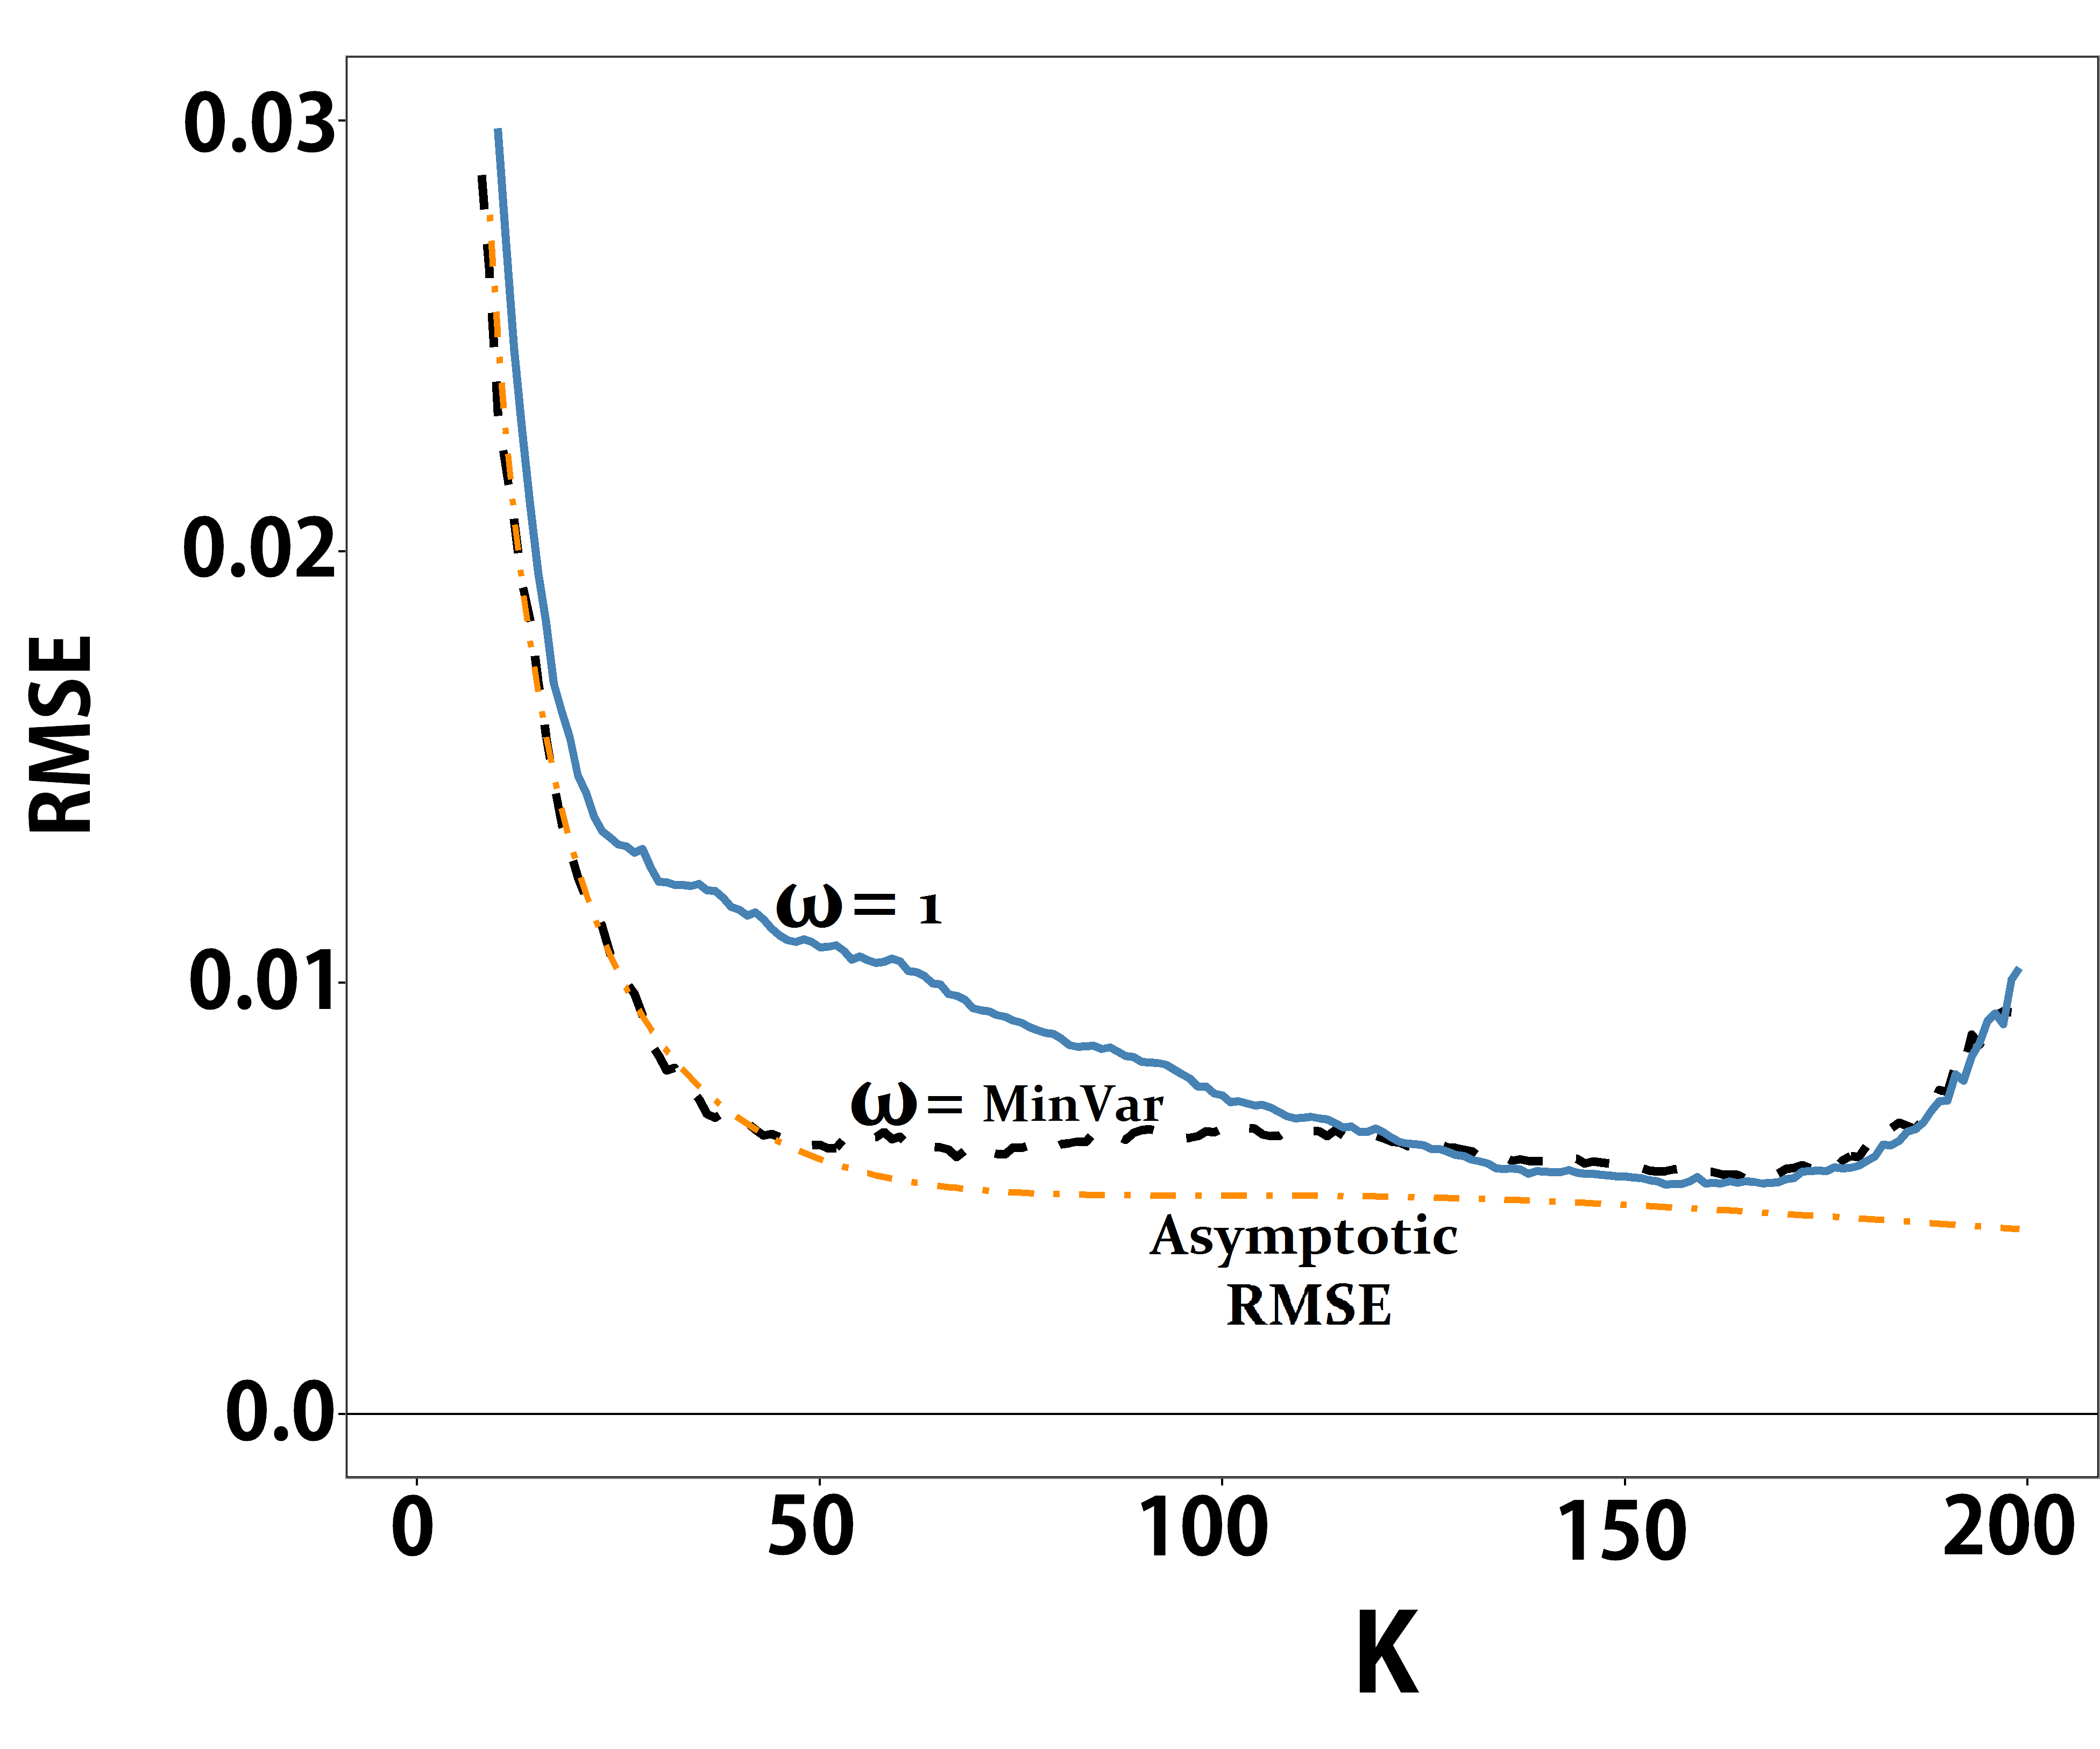
\includegraphics[width=65mm]{./plots/paper1/mseFrechetKappa.png}
		\end{subfigure}
		\bigskip
		\begin{subfigure}[h]{0.40\linewidth}
			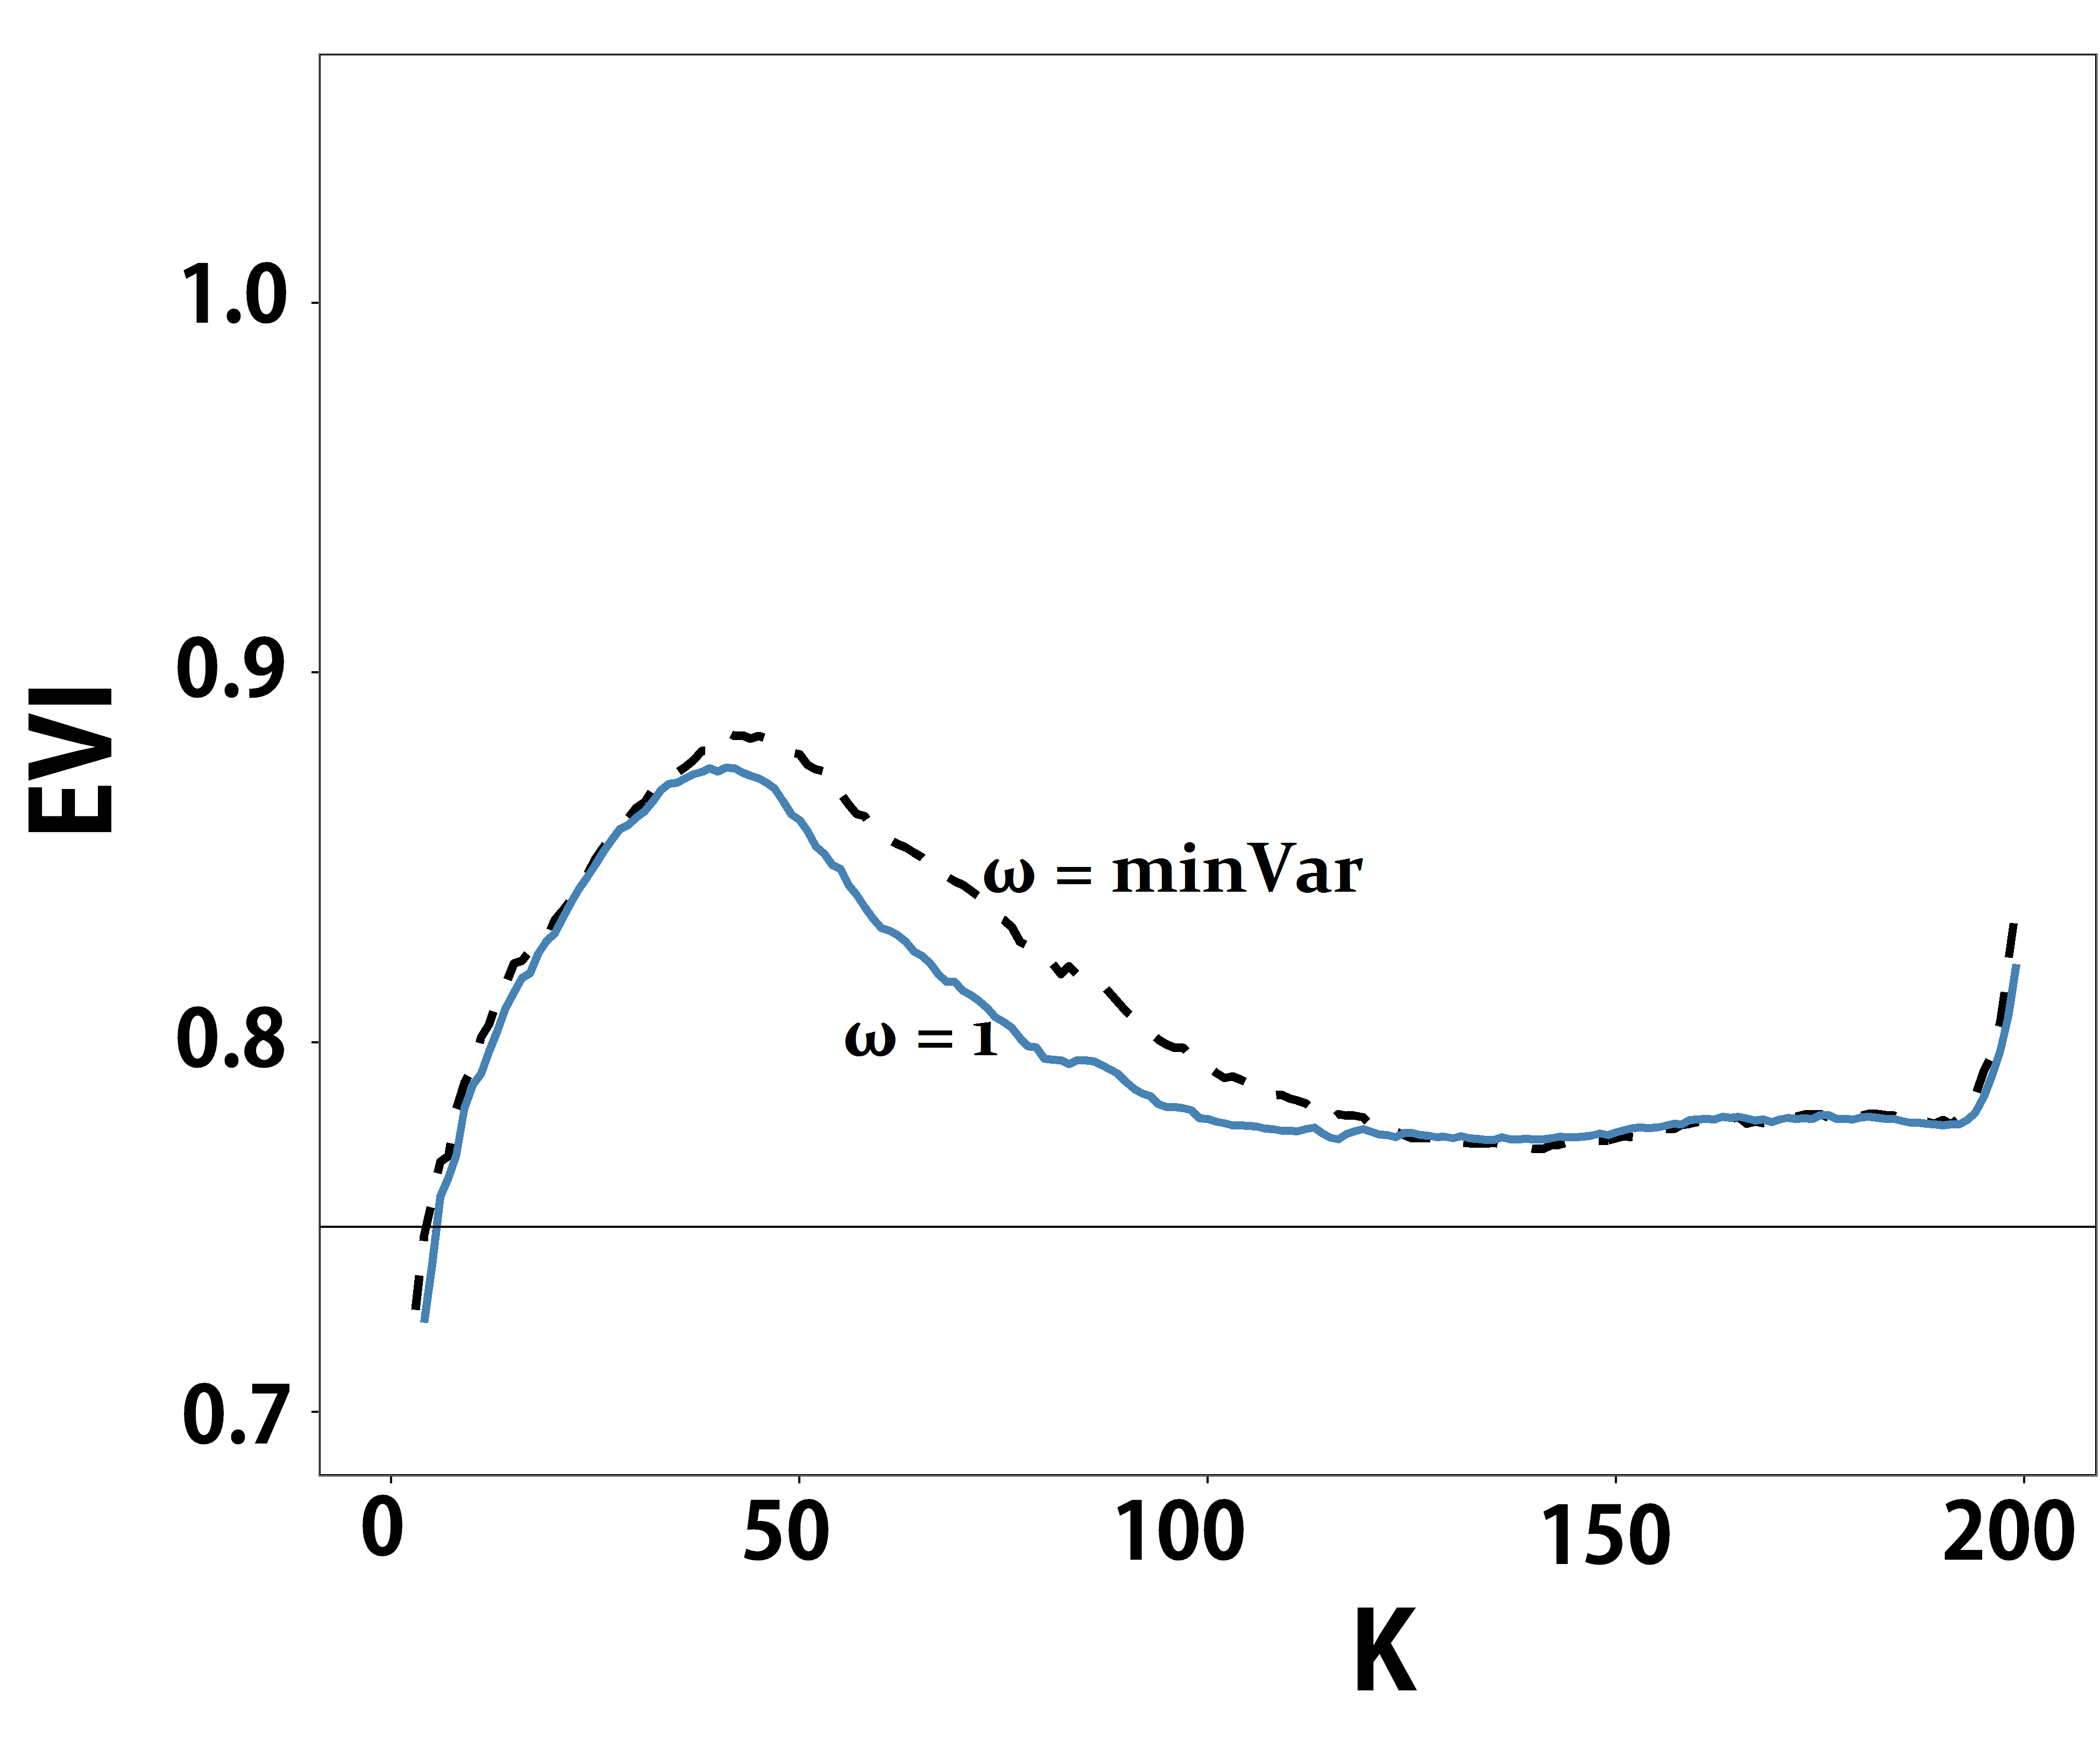
\includegraphics[width=65mm]{./plots/paper1/eviBurrKappa.png}
		\end{subfigure}
		\hspace{\fill}
		\begin{subfigure}[h]{0.40\linewidth}
			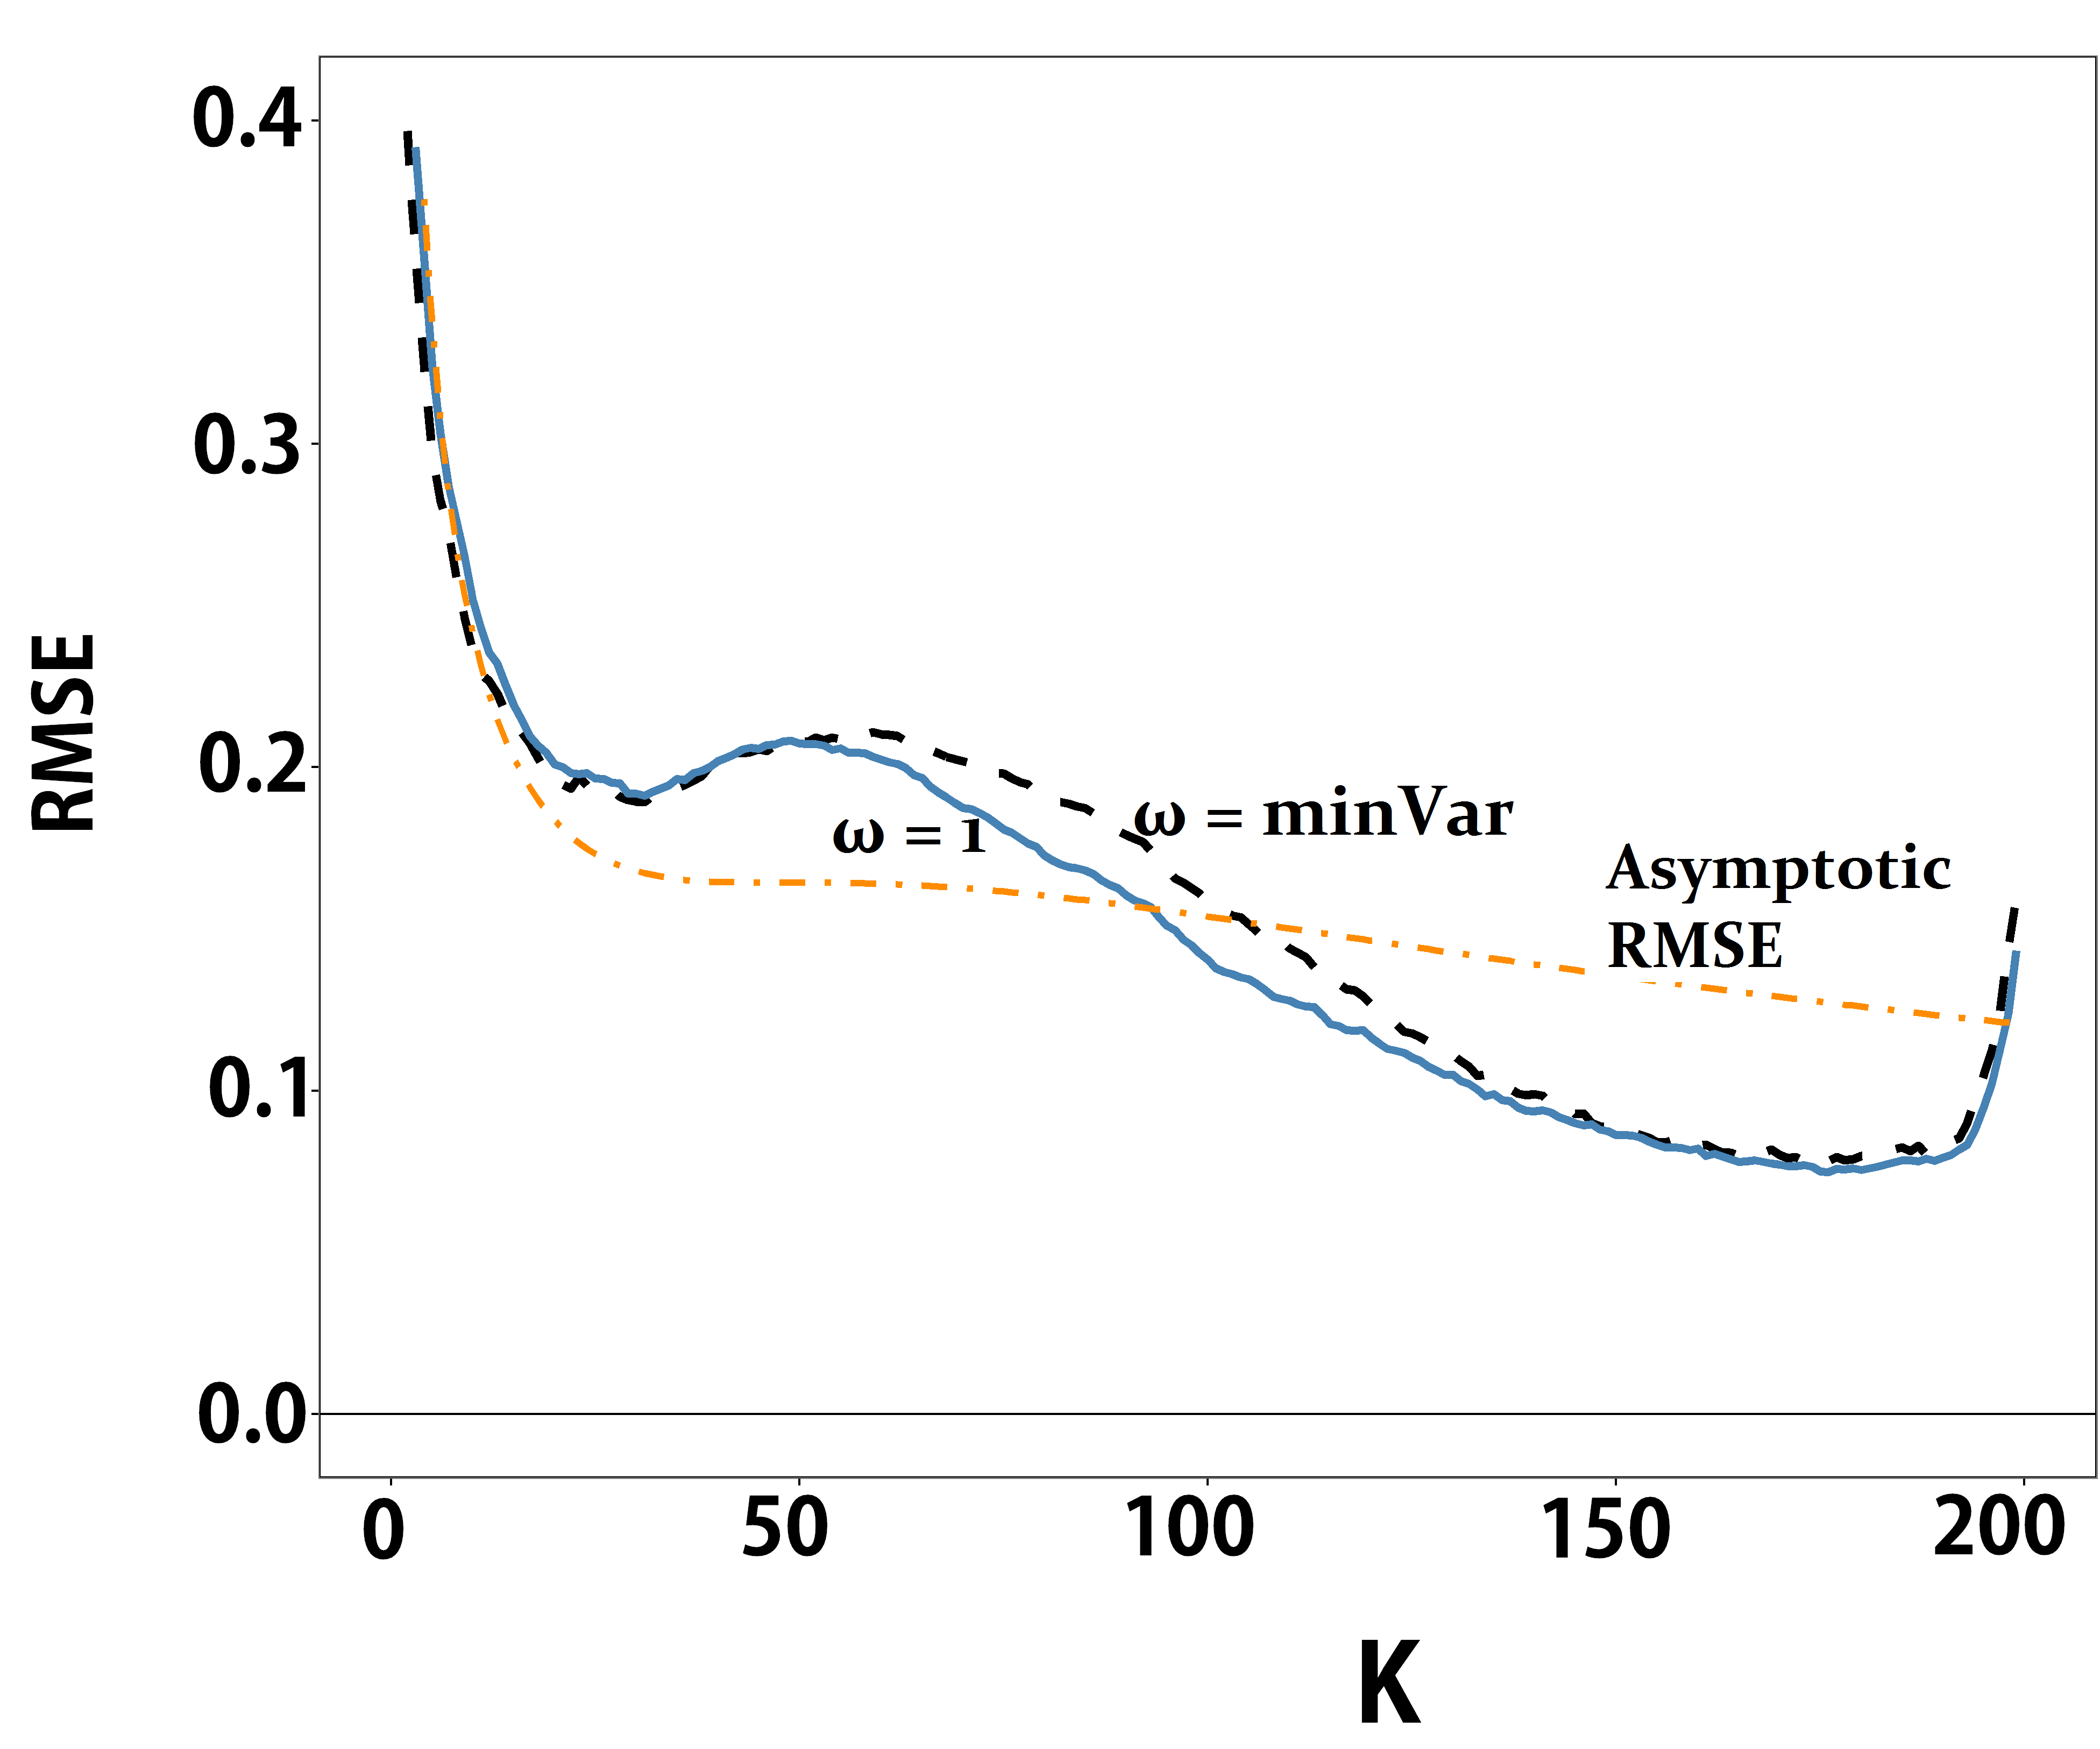
\includegraphics[width=65mm]{./plots/paper1/mseBurrKappa.png}
		\end{subfigure}
		\caption{Bias (left) and root mean squared error (right) in case of the \textbf{Fr\'echet distribution} with $\gamma=0.5$ (top) and Burr distribution with $\gamma=0.75$ (bottom) for sample size $n=200$ comparing  the penalised ML estimator $\hat{\gamma}^P_{k}(1)$ with $\omega=1$, $\omega = \omega_{mv}$ from \eqref{minvar}, and the optimal asymptotic RMSE from \eqref{xisqdiff} replacing $\lambda$ by $C_a\sqrt{k}(k/n)^{-\rho}$.}
		\label{paper1:fig5}
	\end{figure}

In order to illustrate the use of the proposed method we consider the Secura Belgian Re data introduced in section 6.2 in \cite{sts626}.  For $k \leq 100$ the penalised ML estimator $\hat{\gamma}^P_{k}(1)$ is quite constant and follows the Hill estimator quite closely. This is in contrast with the EPD-ML estimates which vary a lot in that region. The Bayesian estimates $\hat{\gamma}^B_{k}(1)$ and CH estimates show somewhat lower estimates. \cite{sts626} concluded that the Hill estimate in this $k$-region is an appropriate choice and the adaptive choice $\hat{k}=98$ was proposed as one of the largest $k$-values in this region. This proposal is also supported by the present analysis, leading to an estimate $\hat{\gamma}^P(1)=0.28$. 
\begin{figure}[h]
	\centering
	\begin{subfigure}[h]{0.45\textwidth}
		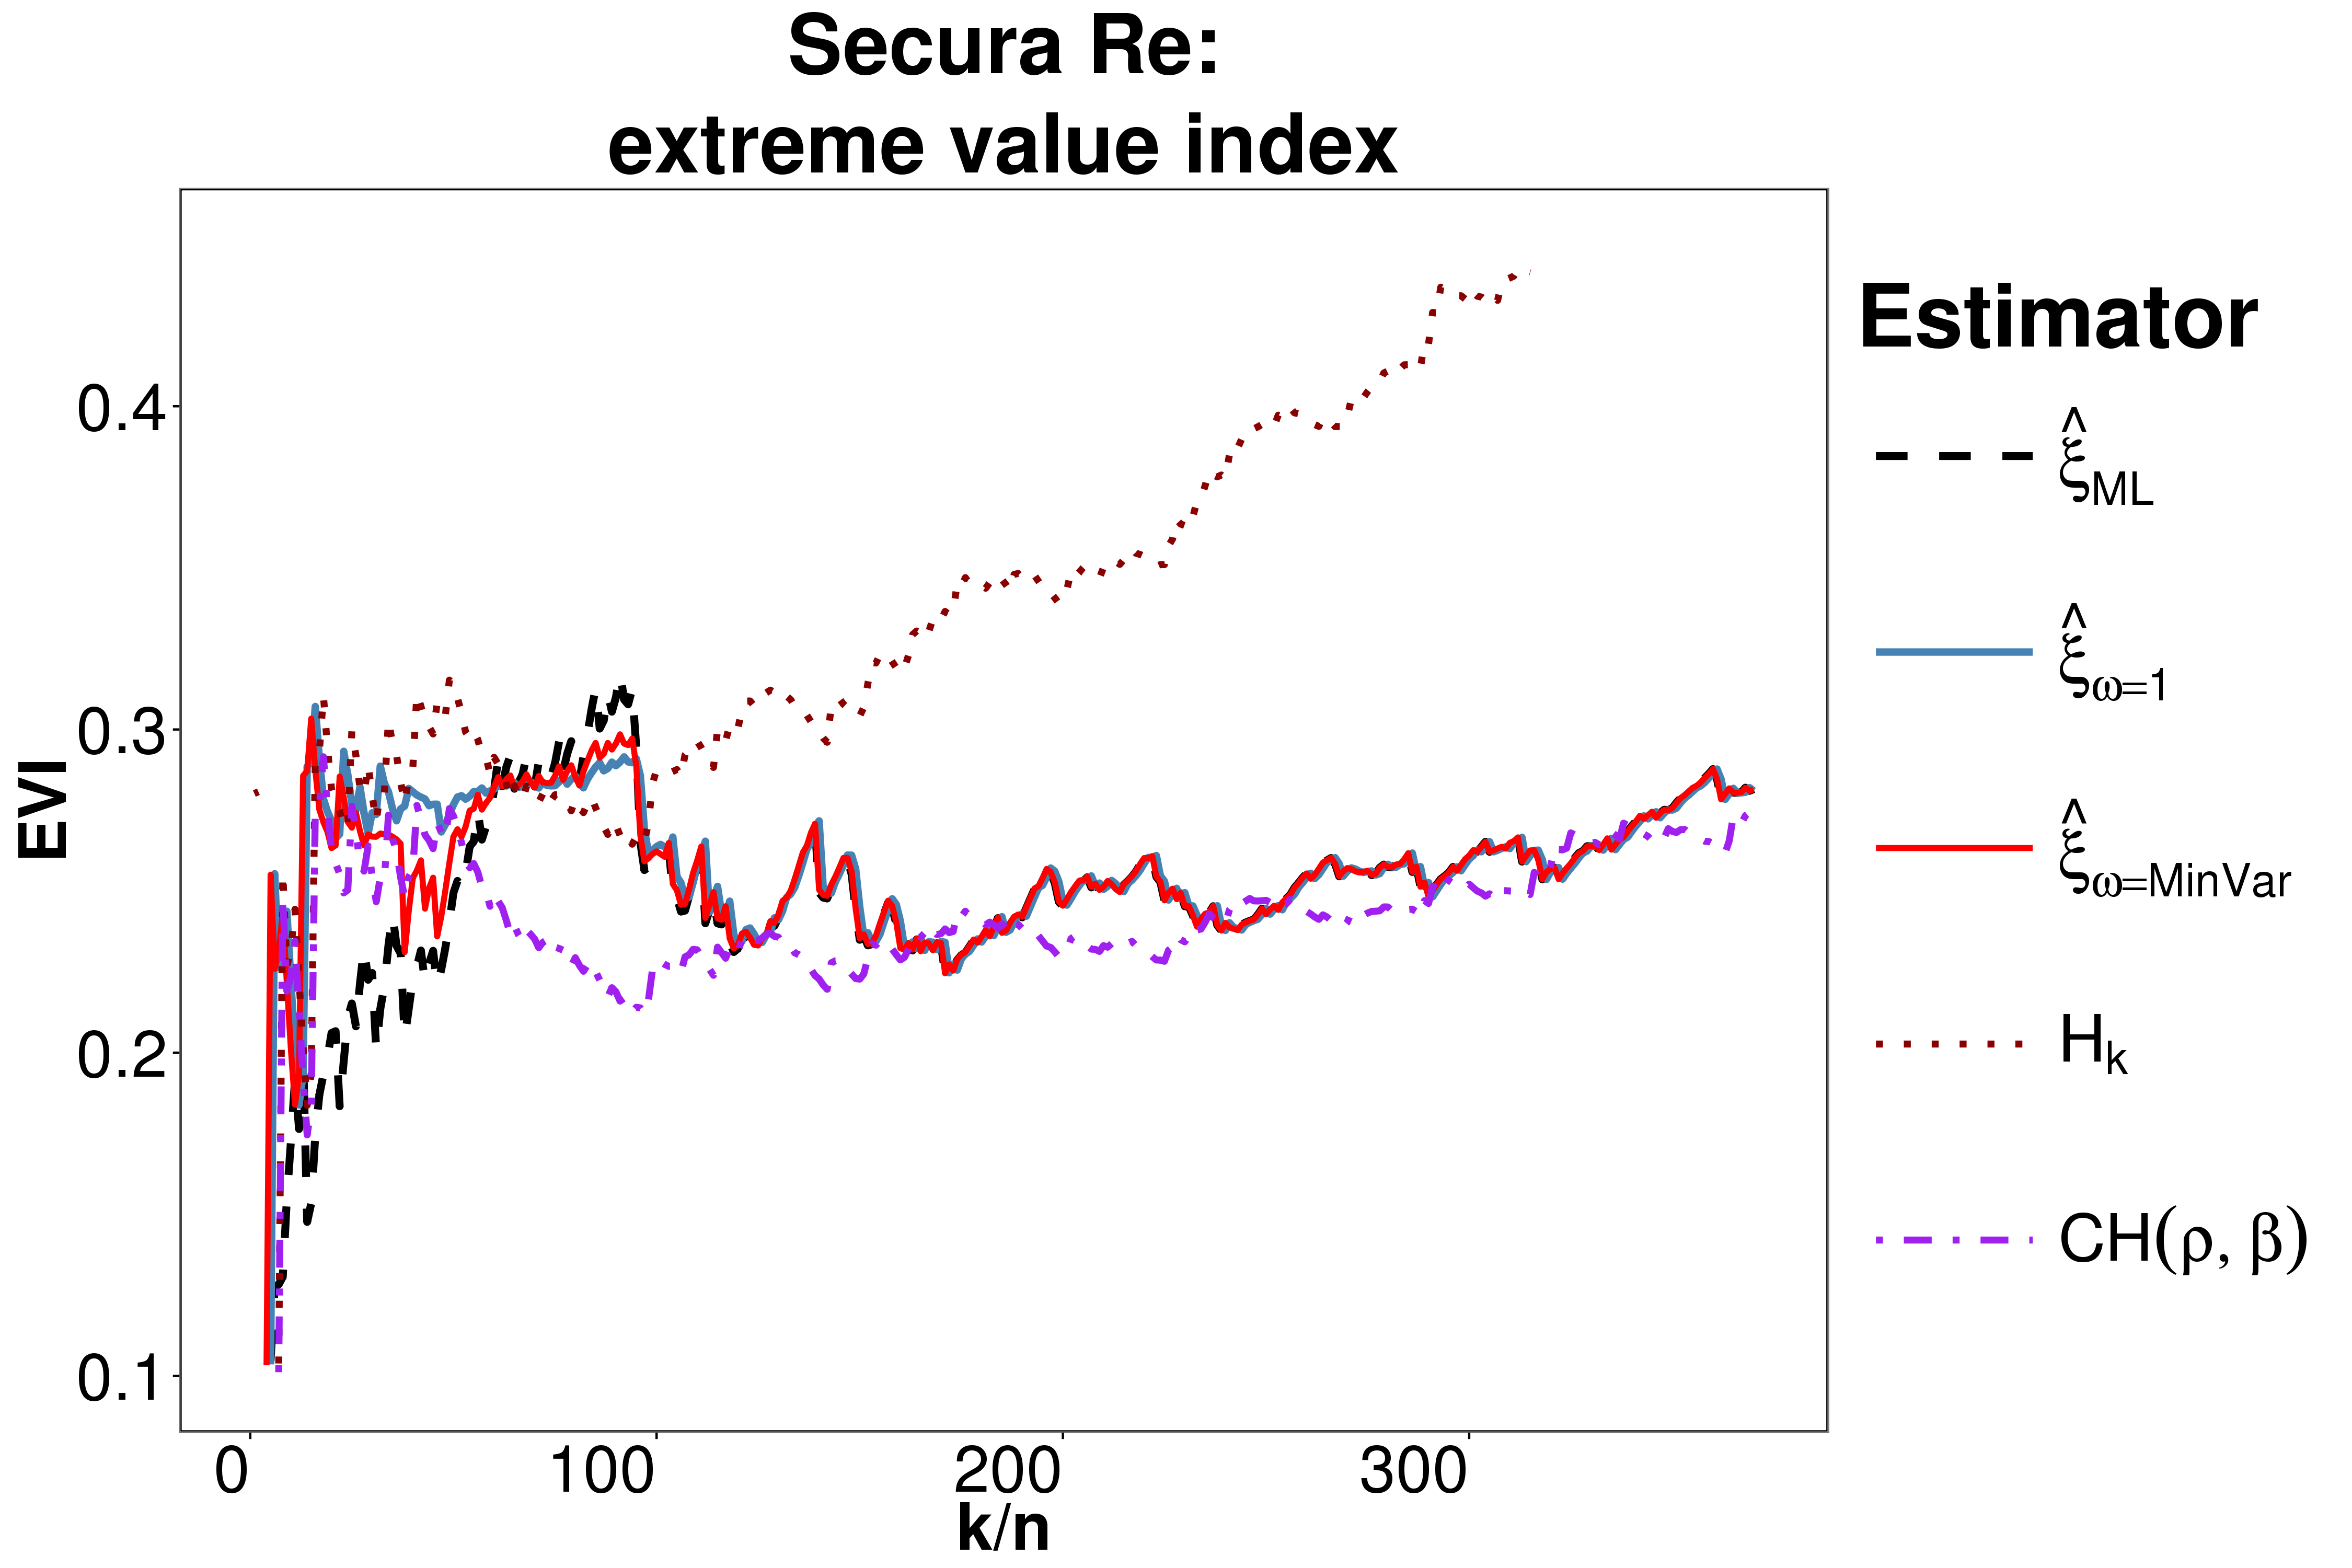
\includegraphics[width=\textwidth]{./plots/paper1/SecuraEVI.png}
	\end{subfigure}
	\hspace{\fill}
	\begin{subfigure}[h]{0.45\textwidth}
		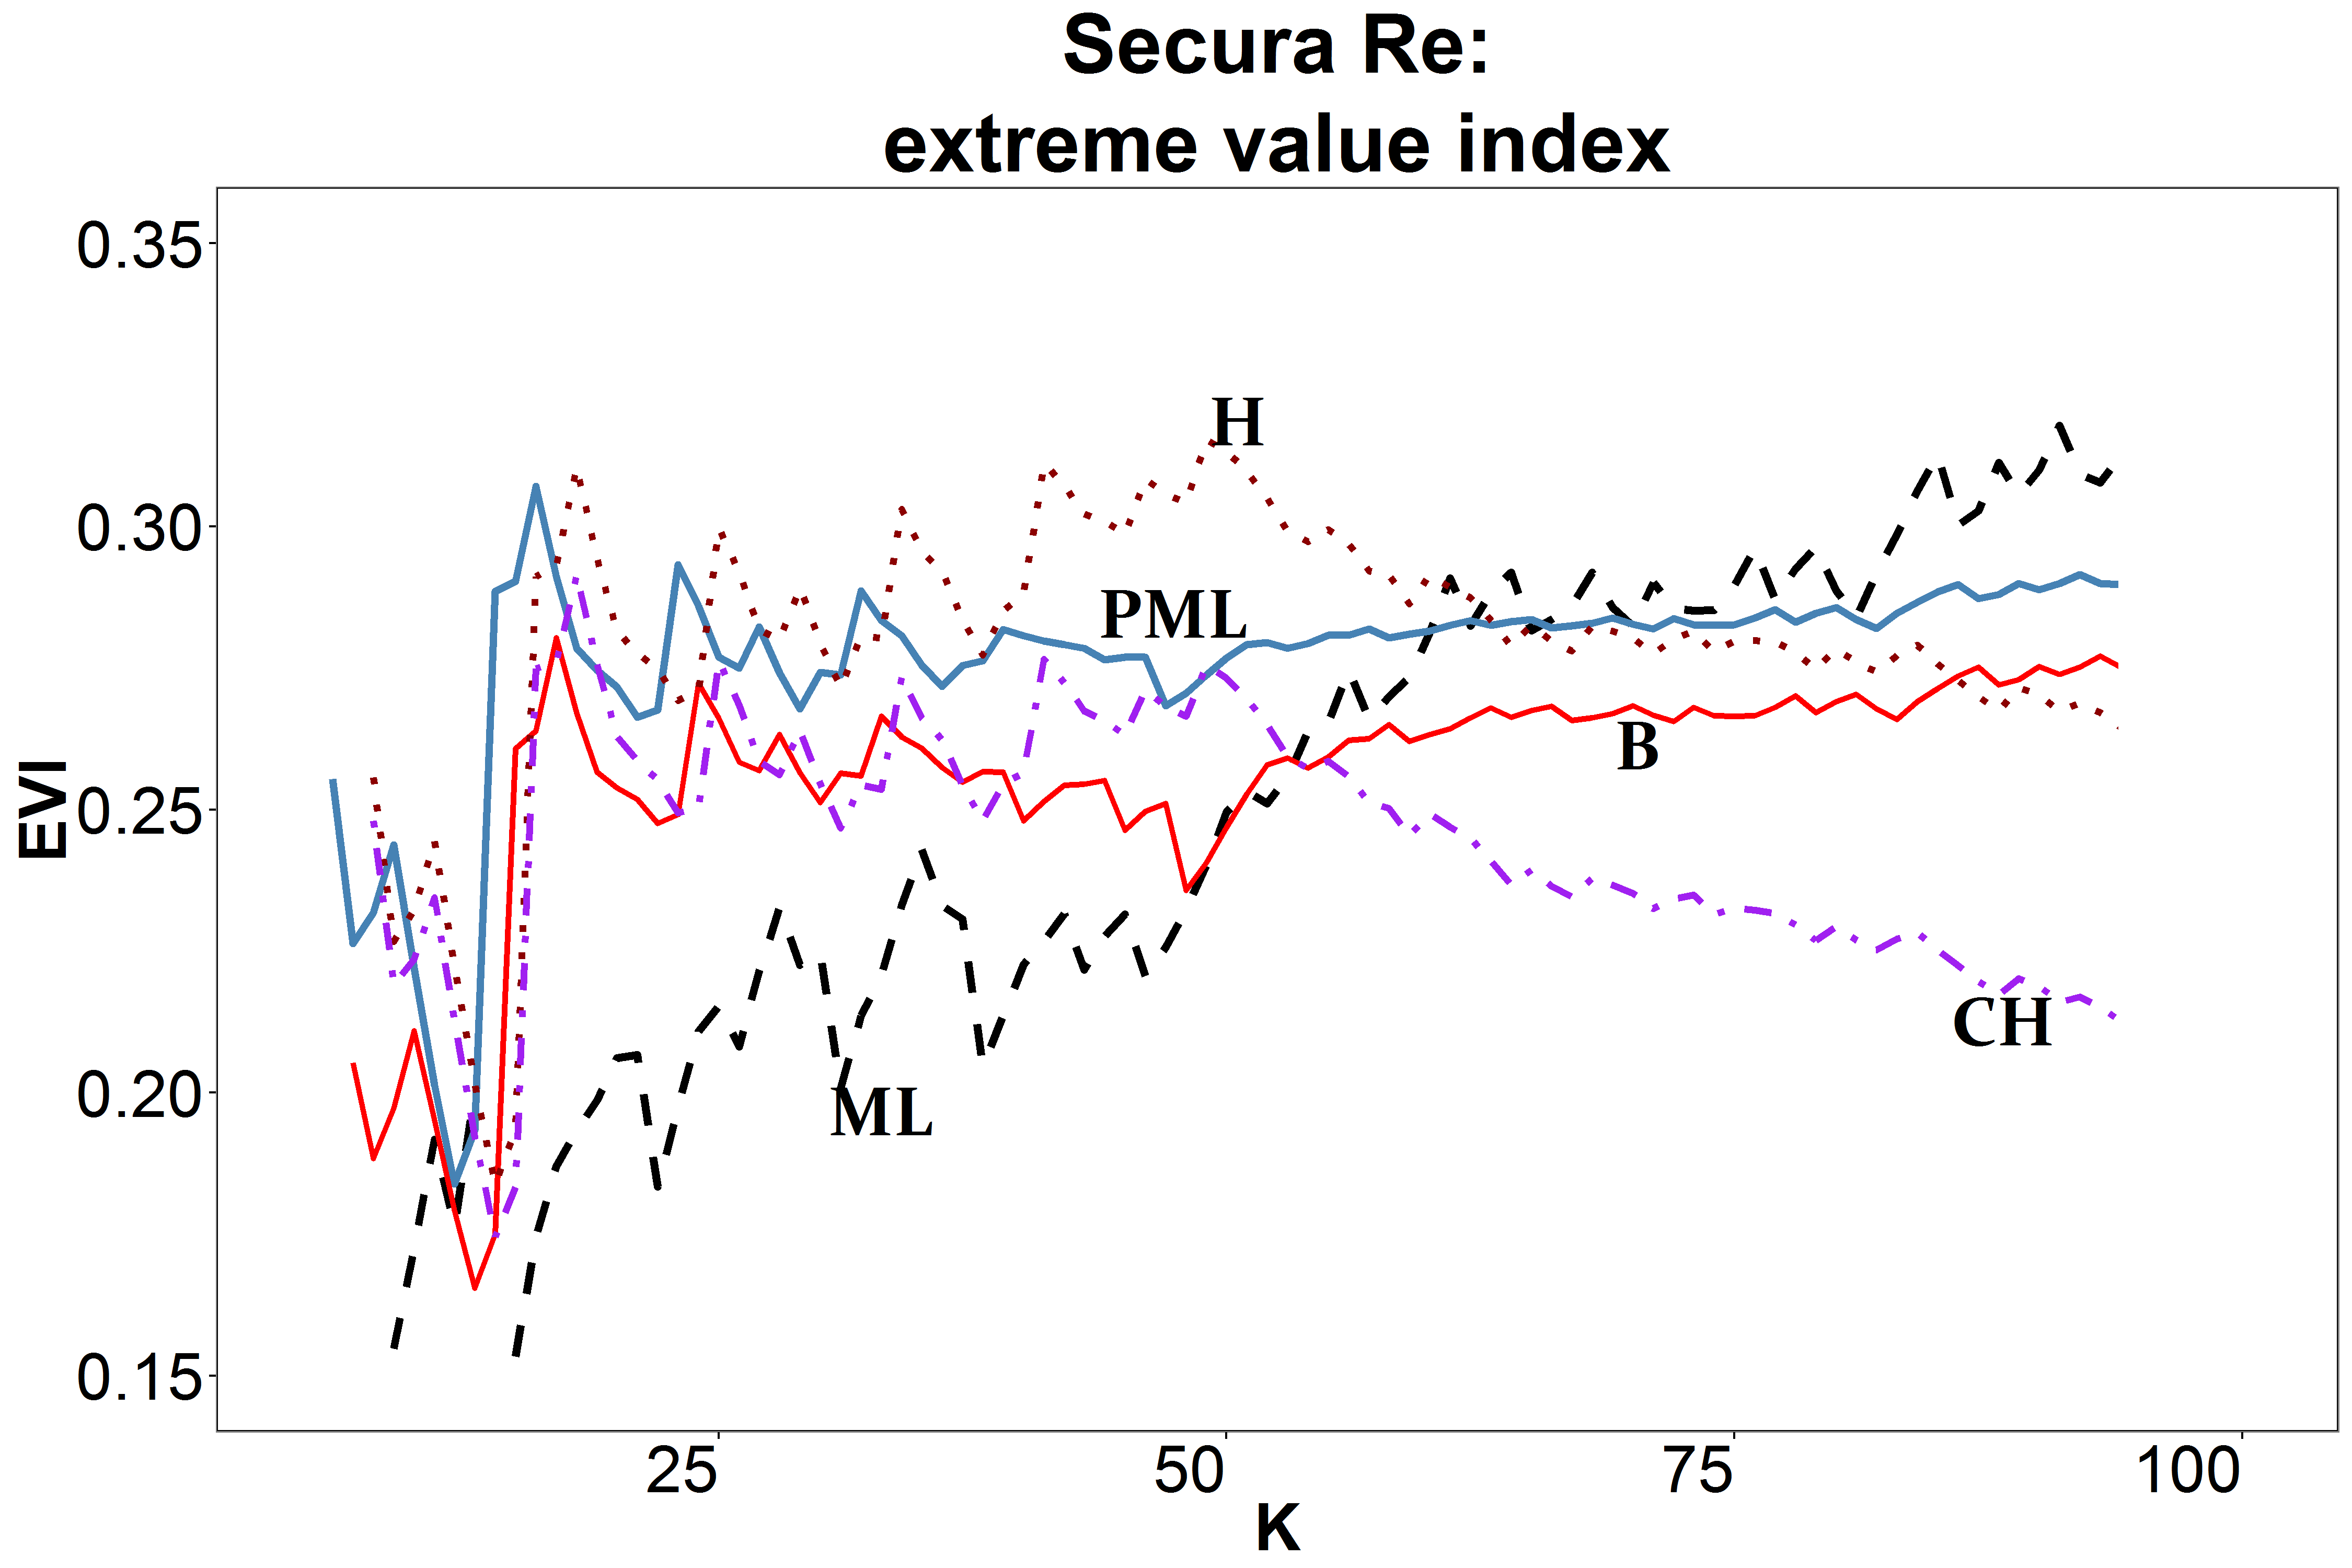
\includegraphics[width=\textwidth]{./plots/paper1/cutSecuraEVI.png}
	\end{subfigure}
	\caption{\footnotesize Estimates of  $\gamma$ for Secura Belgian Re data set: results for the Hill estimator (H), the EPD-ML estimator $\hat{\gamma}_{k}^{ML}$ (ML), the penalised ML estimator $\hat{\gamma}^P_{k}(1)$ with $\omega=1$ (PML), the Bayesian estimator $\hat{\gamma}^B_{k}(1)$ with $\omega=1$ (B), and the minimum variance reduced bias estimator $CH_k$ (CH) (left), focused plot for $k=1,\ldots,100$ (right).}
	\label{Secura} 	
\end{figure}
\\
\section{Chapter conclusion}
We introduced the use of shrinkage estimators in tail estimation, in order to obtain bias reduction jointly with good MSE behaviour. Shrinkage estimators can be obtained through a penalised ML approach, or through a Bayesian implementation. For larger thresholds the proposed estimators follow the behaviour of the classical Hill estimator with small bias and minimal variance, while the new estimators are never worse than the corresponding bias reduced ML estimators without penalisation. The simulated MSE results are competitive with those of other bias reduced estimators. In contrast to existing minimum variance bias reduced estimators we only use second order slow variation conditions.

\begin{subappendices}
\section{Derivation of the expressions of ($\gammab,\db$).} 
First consider the asymptotic approximations of the penalised ML estimator of $\gamma$ based on maximisation of \eqref{loglp}. From \eqref{logl}-\eqref{loglp} using expansions in $\delta \to 0$ 
we obtain 
\begin{eqnarray*}
	{1 \over k}\log l_{pen}(\gamma,\delta |{\bf y}) &=& 
	-\left(1+{1 \over k}\right) \log \gamma -{1 \over k}\left(1+\gamma\right) -\left(\frac{1}{\gamma}+1\right){1 \over k}\sum_{j=1}^k\log y_{j,k} \\
	&& -\delta\left({1 \over \gamma} + 1\right){1 \over k}\sum_{j=1}^k (1-y_{j,k}^{\tau})
	+ \delta {1 \over k}\sum_{j=1}^k (1- (1+\tau)y_{j,k}^{\tau})\\
	&&- {\omega \delta^2 \over 2k\sigma_{k,n}^2}
	+\left({\delta^2 \over 2}\right)\left({1  \over \gamma} +1\right){1 \over k}\sum_{j=1}^k (1-y_{j,k}^{\tau})^2
	- {\delta^2 \over 2} {1 \over k}\sum_{j=1}^k (1- (1+\tau)y_{j,k}^{\tau})^2 \\
	&&+ O(\delta^3) + c,
\end{eqnarray*}
where $c$ is a constant only depending on $\sigma_{k,n}^2$ and $\tau$. Note that ${1 \over k}\sum_{j=1}^k\log y_{j,k}=H_{k,n}$. Then the score functions admit the following expansions in $\delta \downarrow 0$ for $j=1,\ldots,k$:
\begin{eqnarray*}
	{\partial \over \partial \gamma}\log l_{pen}(\gamma,\delta |y_{j,k}) &=& -{1 \over \gamma} + {1 \over \gamma^2} \log y_{j,k}
	+{\delta \over \gamma^2}(1-y_{j,k}^{\tau})
	+ O(\delta^2), \\
	{\partial \over \partial \delta}\log l_{pen}(\gamma,\delta |y_{j,k}) &=& -{1 \over \gamma}\left( 1- (1-\gamma\tau) y_{j,k}^{\tau} \right) -{\omega\delta \over k\sigma^2_{k,n}}\\
	&&
	+ {\delta \over \gamma} \left( 1- 2(1-\gamma\tau) y_{j,k}^{\tau} 
	+ (1-2\gamma\tau-\gamma\tau^2) y_{j,k}^{2\tau}\right)+ O(\delta^2).
\end{eqnarray*}

\vspace{0.4cm}\noindent 
{\it Derivation of Theorem \ref{theorem11}.}
Note that as $k,n \to \infty$, $k/n \to 0$ and $\sqrt{k} a(n/k) \to \lambda$, we also have $k\sigma^2_{k,n} \to \lambda^2 C_a^{-2}$. Also as $\sqrt{k} a(n/k) \to \lambda$ we find using
$E_{k,n}(s) \to 1/(1-\gamma s)$ (see Theorem A.1 in Beirlant et al., 2009) that
$$
D^{P}_{k,n} = -{\gamma C_a^2 \over \lambda^2} 
+ {\rho^4 \over \gamma (1-2\rho)(1-\rho)^2} + o_p(1).
$$
Then, proceeding as in the proof of Theorem 3.1 in Beirlant et al. (2009), we obtain with $\Gamma_{k,n} = \sqrt{k}( H_{k,n}-\gamma)$, $\mathbb{E}_{k,n}(s) =\sqrt{k}(E_{k,n}(s)-{1\over 1-\gamma s })$ ($s<0$), that
\begin{eqnarray*}
	\sqrt{k} \left( \gammab-\gamma \right)&=&
	\sqrt{k} \left( H_{k,n}-\gamma - \db {\rho \over 1-\rho} \right) 
	\\
	&=& \Gamma_{k,n}-{\rho \over 1-\rho}\sqrt{k}\db \\
	&=& \Gamma_{k,n}\left(1+ {\rho^2 \over \gamma(1-\rho^2)}
	{1 \over \gamma C_a^2/\lambda^2+ \rho^4/\gamma(1-2\rho)(1-\rho)^2} \right) \\
	&&- {\rho \over \gamma C_a^2/\lambda^2+\rho^4/\gamma(1-2\rho)(1-\rho)^2} \mathbb{E}_{k,n}(\hat\tau) +o_p(1)\\
	&=& \Gamma_{k,n} \left( 1+ {\rho^2 (1-2\rho)\over \zeta +\rho^4}\right) + 
	\mathbb{E}_{k,n}(\hat\tau)\left( {(-\rho)\gamma(1-2\rho)(1-\rho)^2 \over \rho^4 + \zeta }\right)+o_p(1).
\end{eqnarray*} 
Using Theorem A.1 in Beirlant et al. (2009), \eqref{Abias} and \eqref{Avar} follow under $\sqrt{k} a(n/k) \to \lambda$.
\label{appendix1}

\section{Optimal $\omega$ minimising the $MSE_{\infty}$}
$$
MSE_{\infty} = (E_{\infty})^2 + \text{VAR}_{\infty}
$$
\begin{eqnarray*}
E_{\infty} = \dfrac{\lambda \rho \left(\zeta C_a^2 \omega \right)}{(1-\rho ) \left(\zeta C_a^2 \omega +\lambda ^2 \rho ^4\right)}\ ,\ \ 
\text{VAR}_{\infty} = \dfrac{\left(\lambda ^4 \xi ^2 \rho ^8\right) \left(\dfrac{C_a^4 \zeta ^2 \omega ^2}{\lambda ^4 \rho ^8}+\dfrac{2 \zeta C_a^2 \omega }{\lambda ^2 \rho ^4}+\left(\dfrac{1-\rho }{\rho }\right)^2\right)}{\left(\zeta C_a^2 \omega +\lambda ^2 \rho ^4\right)^2}
\end{eqnarray*}

\begin{eqnarray*}
MSE_{\infty}= \dfrac{\left(\lambda ^4 \xi ^2 \rho ^8\right) \left(\dfrac{C_a^4 \zeta ^2 \omega ^2}{\lambda ^4 \rho ^8}+\dfrac{2 \zeta C_a^2 \omega }{\lambda ^2 \rho ^4}+\left(\dfrac{1-\rho }{\rho }\right)^2\right)}{\left(\zeta C_a^2 \omega +\lambda ^2 \rho ^4\right)^2}+\left(\dfrac{\lambda \rho \left(\zeta C_a^2 \omega \right)}{(1-\rho ) \left(\zeta C_a^2 \omega +\lambda ^2 \rho ^4\right)}\right)^2
\end{eqnarray*}

Where $\zeta = \xi^2(1-2\rho)(1-\rho)^2$

\begin{eqnarray*}
\partial_{\omega}(MSE_{\infty})&=&\dfrac{2 C_a^2 \zeta \lambda ^2 \xi ^2 \rho ^4}{\left(C_a^2 \zeta \omega +\lambda ^2 \rho ^4\right)^2}-\dfrac{2 C_a^2 \zeta \lambda ^4 \xi ^2 \rho ^8}{\left(C_a^2 \zeta \omega +\lambda ^2 \rho ^4\right)^3}+\dfrac{4 C_a^2 \zeta \lambda ^4 \xi ^2 \rho ^7}{\left(C_a^2 \zeta \omega +\lambda ^2 \rho ^4\right)^3}\\&-&\dfrac{2 C_a^2 \zeta \lambda ^4 \xi ^2 \rho ^6}{\left(C_a^2 \zeta \omega +\lambda ^2 \rho ^4\right)^3}-\dfrac{2 C_a6 \zeta ^3 \xi ^2 \omega ^2}{\left(C_a^2 \zeta \omega +\lambda ^2 \rho ^4\right)^3}-\dfrac{2 C_a6 \zeta ^3 \lambda ^2 \rho ^2 \omega ^2}{(1-\rho )^2 \left(C_a^2 \zeta \omega +\lambda ^2 \rho ^4\right)^3}\\&-&\dfrac{4 C_a^4 \zeta ^2 \lambda ^2 \xi ^2 \rho ^4 \omega }{\left(C_a^2 \zeta \omega +\lambda ^2 \rho ^4\right)^3}+\dfrac{2 C_a^4 \zeta ^2 \xi ^2 \omega }{\left(C_a^2 \zeta \omega +\lambda ^2 \rho ^4\right)^2}+\dfrac{2 C_a^4 \zeta ^2 \lambda ^2 \rho ^2 \omega }{(1-\rho )^2 \left(C_a^2 \zeta \omega +\lambda ^2 \rho ^4\right)^2}
\end{eqnarray*}

\begin{eqnarray*}
\partial_{\omega}(MSE_{\infty})=&\dfrac{\lambda ^4 \xi ^2 \rho ^8 \left(\dfrac{2 C_a^4 \zeta ^2 \omega }{\lambda ^4 \rho ^8}+\dfrac{2 \zeta C_a^2}{\lambda ^2 \rho ^4}\right)}{\left(\zeta C_a^2 \omega +\lambda ^2 \rho ^4\right)^2}-\dfrac{2 \zeta C_a^2 \lambda ^4 \xi ^2 \rho ^8 \left(\dfrac{C_a^4 \zeta ^2 \omega ^2}{\lambda ^4 \rho ^8}+\dfrac{2 \zeta C_a^2 \omega }{\lambda ^2 \rho ^4}+\dfrac{(1-\rho )^2}{\rho ^2}\right)}{\left(\zeta C_a^2 \omega +\lambda ^2 \rho ^4\right)^3}\\&-\dfrac{2 \zeta C_a^6 \lambda \rho ^2 \omega ^2}{(1-\rho )^2 \left(\zeta C_a^2 \omega +\lambda ^2 \rho ^4\right)^3}+\dfrac{2 \zeta C_a^4 \lambda \rho ^2 \omega }{(1-\rho )^2 \left(\zeta C_a^2 \omega +\lambda ^2 \rho ^4\right)^2}
\end{eqnarray*}

Which simplifies to:
\begin{eqnarray*}
=\dfrac{2 C_a^2 \zeta \lambda ^4 \xi ^2 (2 \rho -1) \rho ^6}{\left(C_a^2 \zeta \omega +\lambda ^2 \rho ^4\right)^3}+\dfrac{2 C_a^4 \zeta ^2 \lambda ^4 \rho ^6 \omega }{(\rho -1)^2 \left(C_a^2 \zeta \omega +\lambda ^2 \rho ^4\right)^3}
\end{eqnarray*}

\begin{eqnarray*}
=\dfrac{2 C_a^2 \zeta \lambda ^4 \rho ^6 \left(C_a^2 \zeta \omega +\xi ^2 (\rho -1)^2 (2 \rho -1)\right)}{(\rho -1)^2 \left(C_a^2 \zeta \omega +\lambda ^2 \rho ^4\right)^3}
\end{eqnarray*}

Set $\partial_{\omega}(MSE_{\infty})=0$ and solve for $\omega$
\begin{eqnarray*}
\omega \to C_a^{-2}*\left(-\dfrac{\xi ^2 (\rho -1)^2 (2 \rho -1)}{\zeta }\right)
\end{eqnarray*}

After substituting $\zeta$ back into the equation we get:
\begin{eqnarray*}
\omega = C_a^{-2} * \left(-\dfrac{(\rho -1)^2 (2 \rho -1)}{(1-2 \rho ) (1-\rho )^2}\right) = C_a^{-2}
\end{eqnarray*}

\begin{eqnarray*}
\partial_{\omega}^2(MSE_{\infty})=&
\dfrac{2 C_a^4 \zeta ^2 \lambda ^4 \rho ^6}{(\rho -1)^2 \left(C_a^2 \zeta \omega +\lambda ^2 \rho ^4\right)^3}-\dfrac{6 C_a^4 \zeta ^2 \lambda ^4 \rho ^6 \left(C_a^2 \zeta \omega +\xi ^2 (\rho -1)^2 (2 \rho -1)\right)}{(\rho -1)^2 \left(C_a^2 \zeta \omega +\lambda ^2 \rho ^4\right)^4}
\end{eqnarray*}

Substituting $\zeta$ and $\omega= C_a^{-2}$ into the equation:

\begin{eqnarray*}
\partial_{\omega}^2(MSE_{\infty})=&&-\dfrac{8 C_a^4 \lambda ^4 \xi ^4 \rho ^{10}}{\left(\xi ^2 (\rho -1)^2 (2 \rho -1)-\lambda ^2 \rho ^4\right)^3}+\dfrac{24 C_a^4 \lambda ^4 \xi ^4 \rho ^9}{\left(\xi ^2 (\rho -1)^2 (2 \rho -1)-\lambda ^2 \rho ^4\right)^3}\\&-&\dfrac{26 C_a^4 \lambda ^4 \xi ^4 \rho ^8}{\left(\xi ^2 (\rho -1)^2 (2 \rho -1)-\lambda ^2 \rho ^4\right)^3}+\dfrac{12 C_a^4 \lambda ^4 \xi ^4 \rho ^7}{\left(\xi ^2 (\rho -1)^2 (2 \rho -1)-\lambda ^2 \rho ^4\right)^3}\\&-&\dfrac{2 C_a^4 \lambda ^4 \xi ^4 \rho ^6}{\left(\xi ^2 (\rho -1)^2 (2 \rho -1)-\lambda ^2 \rho ^4\right)^3}
\end{eqnarray*}

\begin{eqnarray*}
=&&\dfrac{2 C_a^4 \lambda ^4 \xi ^4 (1-2 \rho )^2 (1-\rho )^4 \rho ^6}{(\rho -1)^2 \left(C_a^2 \xi ^2 (1-\rho )^2 (1-2 \rho ) \omega +\lambda ^2 \rho ^4\right)^3}\\&-&\dfrac{6 C_a^4 \lambda ^4 \xi ^4 (1-2 \rho )^2 (1-\rho )^4 \rho ^6 \left(C_a^2 \xi ^2 (1-2 \rho ) (1-\rho )^2 \omega +\xi ^2 (\rho -1)^2 (2 \rho -1)\right)}{(\rho -1)^2 \left(C_a^2 \xi ^2 (1-\rho )^2 (1-2 \rho ) \omega +\lambda ^2 \rho ^4\right)^4}
\end{eqnarray*}

\begin{eqnarray*}
=&&-\dfrac{2 C_a^4 \lambda ^4 \xi ^4 (1-2 \rho )^2 (\rho -1)^2 \rho ^6}{\left(\xi ^2 (\rho -1)^2 (2 \rho -1)-\lambda ^2 \rho ^4\right)^3}
\end{eqnarray*}

This leads to the following series expansion around zero
\begin{eqnarray*}
&-\dfrac{2 \lambda ^4 \left(C_a^4 \rho ^6\right)}{\xi ^2 (\rho -1)^4 (2 \rho -1)}+O\left(\lambda ^5\right) \\&\approx
\dfrac{2 C_a^4 \lambda ^4 \rho ^6}{\xi ^2 (\rho -1)^4 (1-2 \rho)} > 0
\end{eqnarray*}Using the fact that $\rho < 0$, we can conclude that $\omega = C_a^{-2}$ is the optimal value that minimises the MSE.
\label{appendix1a}
\newpage
\section{Algorithm to estimate $\rho$}
	In this section we provide the algorithm of \cite{alves2003new} used to estimate $\rho$.
	\begin{enumerate}
			\item Given a sample ($X_1,X_2,...,X_n$), plot the estimates of \begin{equation}\label{pkt}
			\hat{\rho}_{k,r}:=\min\{0,\dfrac{3(T^{(\tau)}_{k,n}-1)}{T^{(\tau)}_{k,n}-3}\},
			\end{equation}for $\tau=0$, where 
			\begin{equation}\label{tau0}
			T_{k,n}:= \dfrac{\left(M_{k,n}^{(1)}\right)^{\tau}-\left(\dfrac{M^{(2)}_{k,n}}{2}\right)^{\tau/2}}{\left(\dfrac{M^{(2)}_{k,n}}{2}\right)^{\tau/2}-\left(\dfrac{M^{(3)}_{k,n}}{6}\right)^{\tau/3}}
			\end{equation}and
			\begin{equation}
			M^{(j)}_{k,n}:=\dfrac{1}{k}\sum_{i\leq k}^{}(\log X_{n-i+1:n}-\log X_{n-k:n})^j, \ \ j \geq 1.
			\end{equation}since $\tau=0$, the notation $a^{b\tau}=b\ln a$ is used and therefore \autoref{tau0} is written as
			\begin{equation}
			T_{k,n}:= \dfrac{\log(M_{k,n}^{(1)})-\dfrac{1}{2}\log\left(\dfrac{M^{(2)}_{k,n}}{2}\right)}{\dfrac{1}{2}\log\left(\dfrac{M^{(2)}_{k,n}}{2}\right)-\dfrac{1}{3}\log\left(\dfrac{M^{(3)}_{k,n}}{6}\right)}
			\end{equation}
			
			\item Consider $\{\hat{\rho}_{k,n}\}_{k\in \mathcal{K}}$ as given in \autoref{pkt} for large $k$, say $k\in \mathcal{K}=([n^{0.990}],[n^{0.999}])$, compute their median, denoted $\rho_\tau$ and work with $\hat{\rho}\equiv\hat{\rho}_{\tau_{0}}:=\hat{\rho}_{k_1}$, with\begin{equation}
			k_1=[n^{0.995}]
			\end{equation}
		\end{enumerate}
		The choice of the level $k_1$ is not very important, we can consider any reasonably large value of $k$ of order $n^{1-\epsilon}$ from some intermediate sequence of integers $k=k(n)$ satisfying $\lim\limits_{n\rightarrow\infty}\sqrt{k}A(n/k)=\infty$. This estimator uses more upper order statistics than the first order parameter $\gamma$.
\label{appendix1b}
\end{subappendices}